\section{Results}\label{sec:Results}
\subsection{Standard Spectral Components}\label{results: standard components}
% \begin{figure}[b!]
    \centering
    % \begin{tabular}[c]{ccc}
    % \begin{subfigure}[c]{0.31\textwidth}
    %     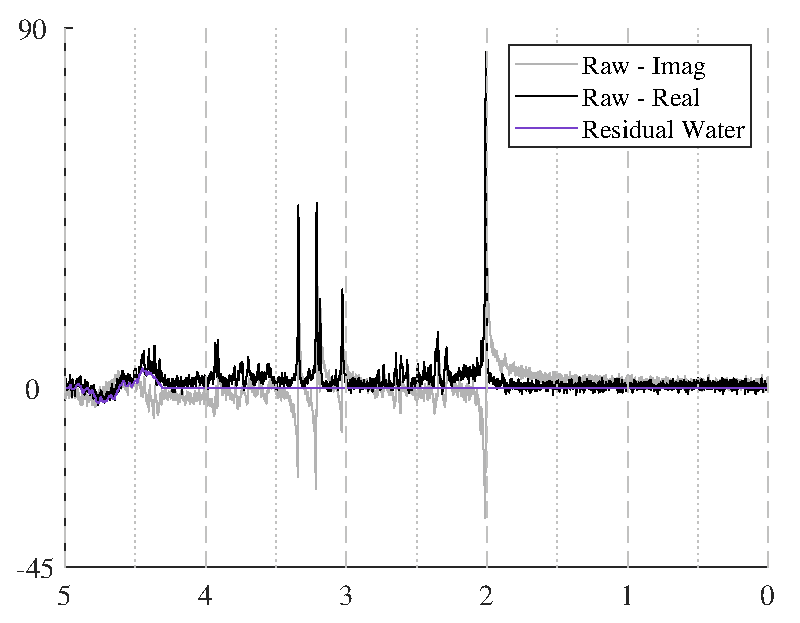
\includegraphics[width=0.93\textwidth]{images/samples_by_artifact/30ms_artifact_samples_lorentzian_1.eps}
    %     \caption{${T_2}^* \times 0.25$}
    %     \vspace{3pt}
    % \end{subfigure}&
    % \begin{subfigure}[c]{0.31\textwidth}
    %     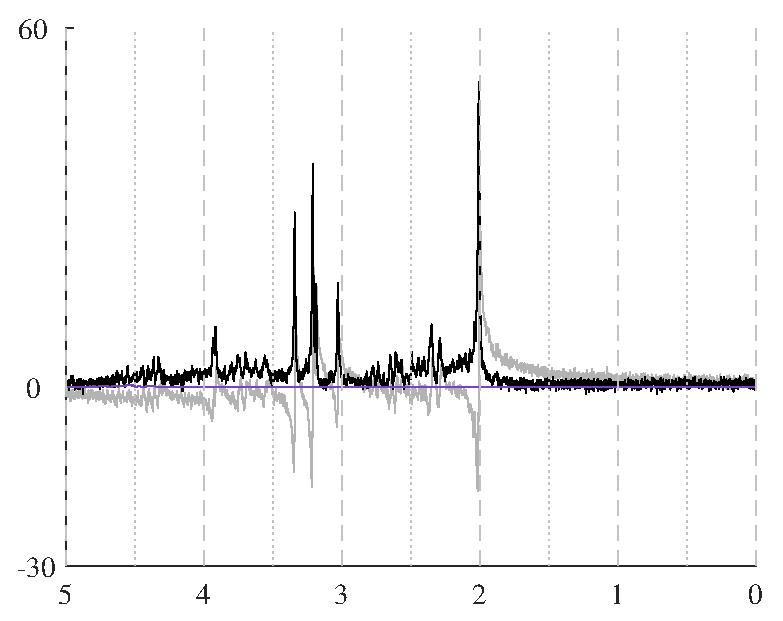
\includegraphics[width=0.93\textwidth]{images/samples_by_artifact/30ms_artifact_samples_lorentzian_2.eps}
    %     \caption{${T_2}^* \times 0.50$}
    %     \vspace{3pt}
    % \end{subfigure}&
    % \begin{subfigure}[c]{0.31\textwidth}
    %     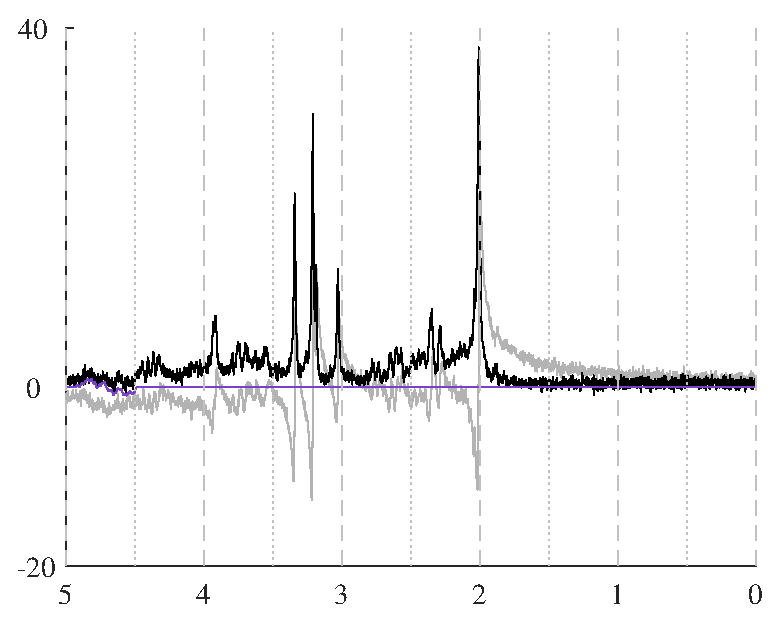
\includegraphics[width=0.93\textwidth]{images/samples_by_artifact/30ms_artifact_samples_lorentzian_3.eps}
    %     \caption{${T_2}^* \times 0.75$}
    %     \vspace{3pt}
    % \end{subfigure}\\
    % \begin{subfigure}[c]{0.31\textwidth}
    %     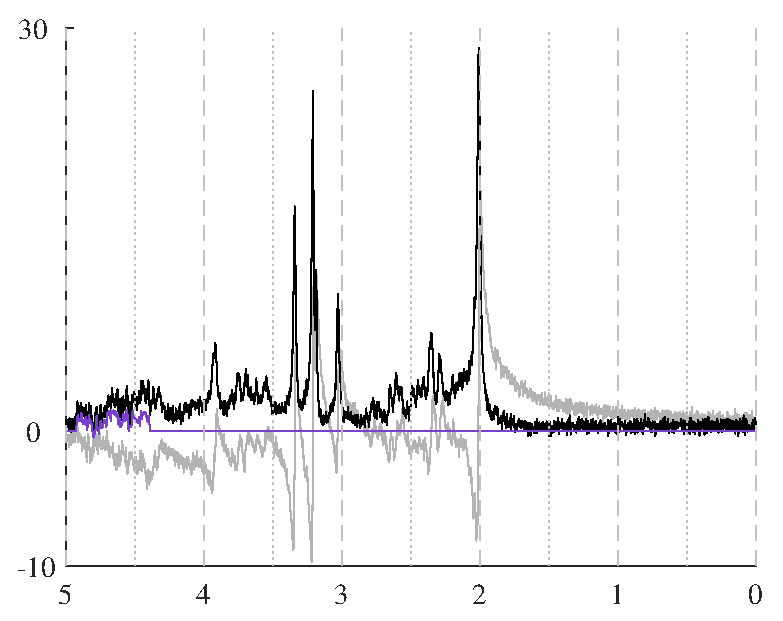
\includegraphics[width=0.93\textwidth]{images/samples_by_artifact/30ms_artifact_samples_lorentzian_4.eps}
    %     \caption{${T_2}^* \times 1.00$}
    %     \vspace{3pt}
    % \end{subfigure}&
    % \begin{subfigure}[c]{0.31\textwidth}
    %     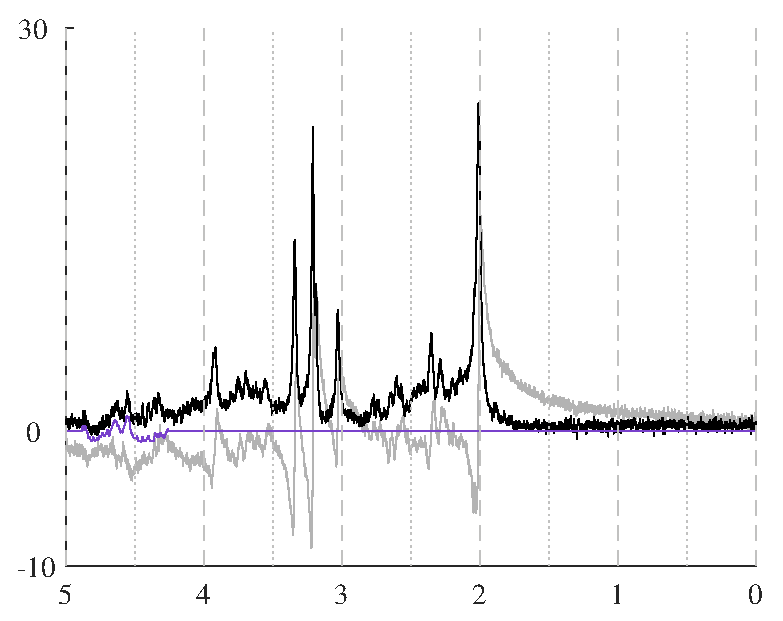
\includegraphics[width=0.93\textwidth]{images/samples_by_artifact/30ms_artifact_samples_lorentzian_5.eps}
    %     \caption{${T_2}^* \times 1.25$}
    %     \vspace{3pt}
    % \end{subfigure}&%
    % \begin{subfigure}[c]{0.31\textwidth}
    %     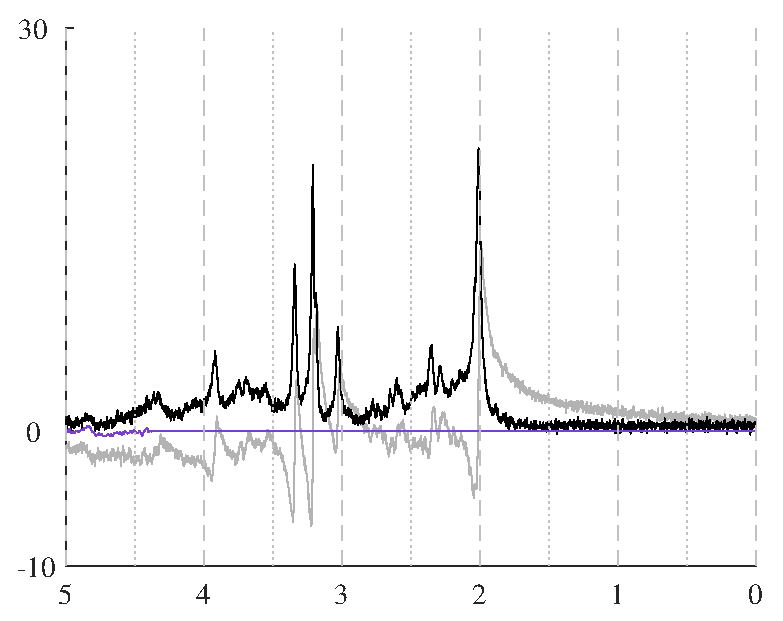
\includegraphics[width=0.93\textwidth]{images/samples_by_artifact/30ms_artifact_samples_lorentzian_6.eps}
    %     \caption{${T_2}^* \times 1.50$}
    %     \vspace{3pt}
    % \end{subfigure}\\
    % \end{tabular}
    \includegraphics[width=\textwidth,keepaspectratio]{images/compiled_figures/MRS_Sim_Figure_8_Lorentzian_Broadening_samples.png}
    \caption{${T_2}^*$ values were fixed and then scaled to represent varying magnitudes of lorentzian broadening. The spectral SNR = 15. No gaussian broadening, baselines, phase offsets, or eddy currents were included.}
    \label{fig:30ms samples lorentzians}
\end{figure}


% \begin{figure}[ht!]
    \centering
    % \begin{tabular}[c]{ccc}
    % \begin{subfigure}[c]{0.31\textwidth}
    %     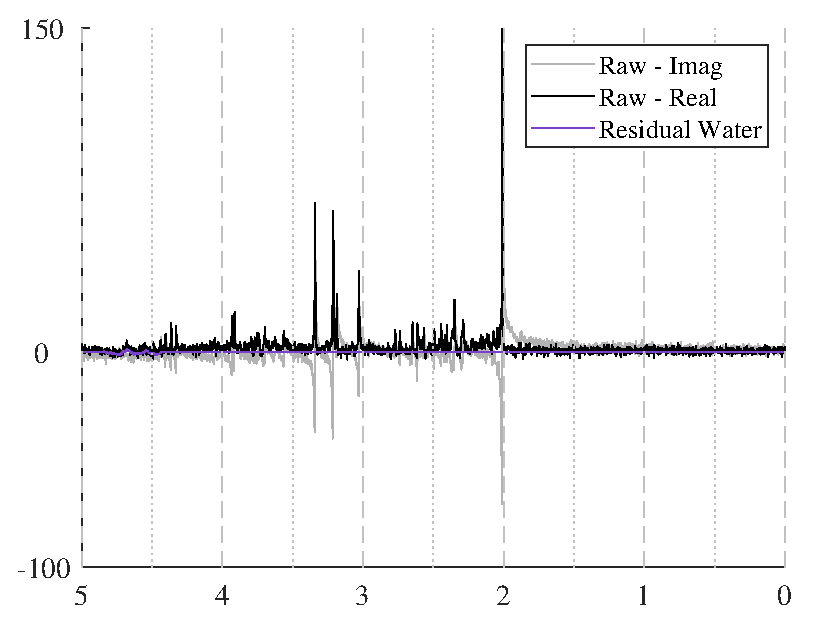
\includegraphics[width=0.93\textwidth]{images/samples_by_artifact/30ms_artifact_samples_gaussian_1.eps}
    %     \caption{Gaussian = 1.0 Hz}
    %     \vspace{3pt}
    % \end{subfigure}&
    % \begin{subfigure}[c]{0.31\textwidth}
    %     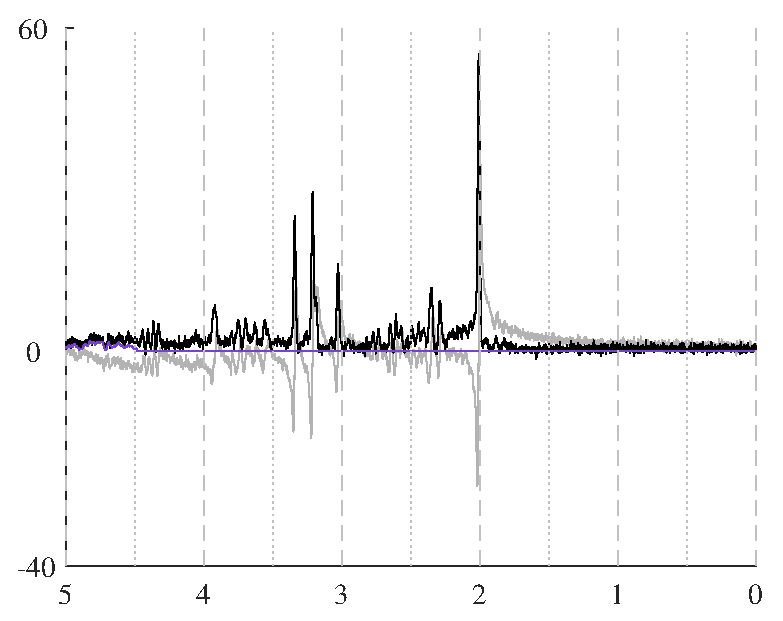
\includegraphics[width=0.93\textwidth]{images/samples_by_artifact/30ms_artifact_samples_gaussian_2.eps}
    %     \caption{Gaussian = 14.9 Hz}
    %     \vspace{3pt}
    % \end{subfigure}&
    % \begin{subfigure}[c]{0.31\textwidth}
    %     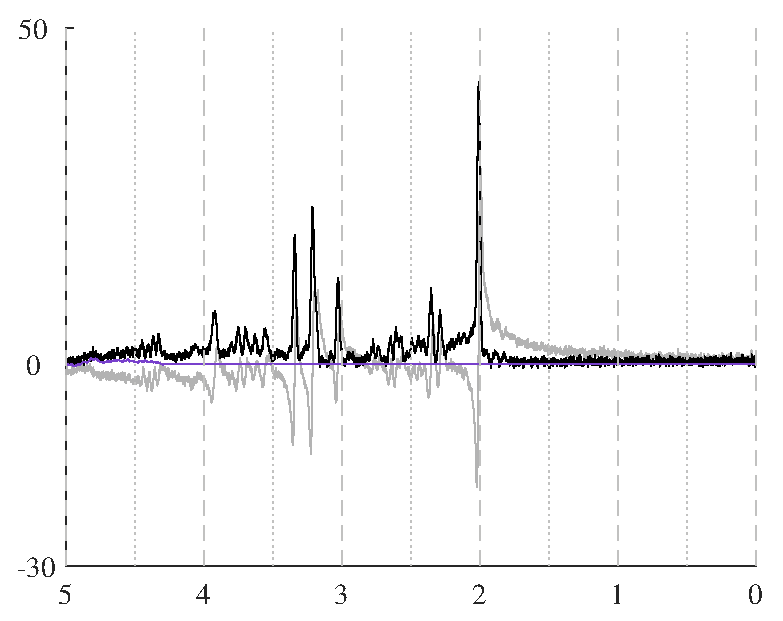
\includegraphics[width=0.93\textwidth]{images/samples_by_artifact/30ms_artifact_samples_gaussian_3.eps}
    %     \caption{Gaussian = 28.8 Hz}
    %     \vspace{3pt}
    % \end{subfigure}\\
    % \begin{subfigure}[c]{0.31\textwidth}
    %     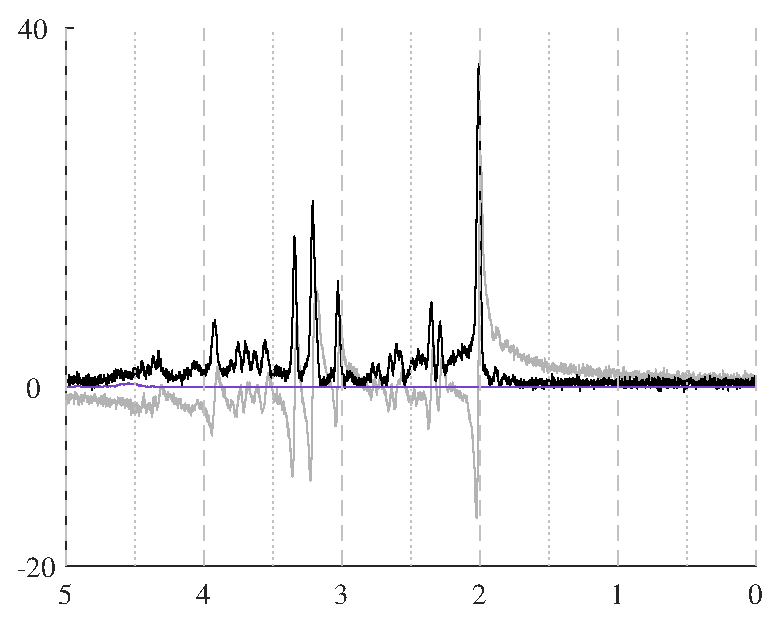
\includegraphics[width=0.93\textwidth]{images/samples_by_artifact/30ms_artifact_samples_gaussian_4.eps}
    %     \caption{Gaussian = 42.8 Hz}
    %     \vspace{3pt}
    % \end{subfigure}&
    % \begin{subfigure}[c]{0.31\textwidth}
    %     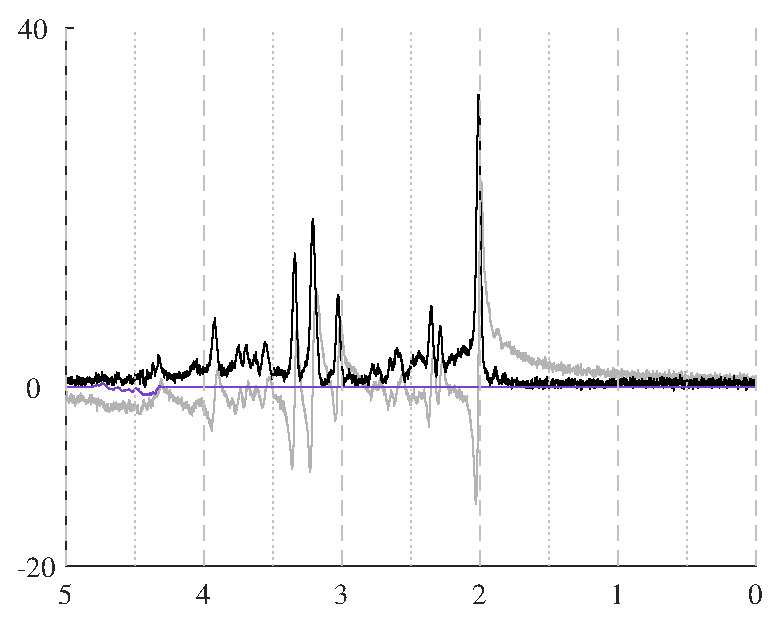
\includegraphics[width=0.93\textwidth]{images/samples_by_artifact/30ms_artifact_samples_gaussian_5.eps}
    %     \caption{Gaussian = 56.7 Hz}
    %     \vspace{3pt}
    % \end{subfigure}&%
    % \begin{subfigure}[c]{0.31\textwidth}
    %     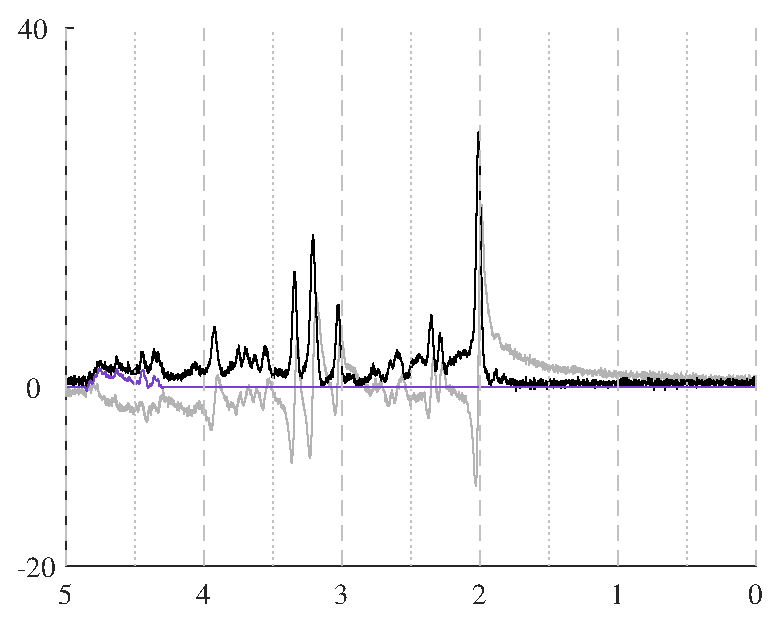
\includegraphics[width=0.93\textwidth]{images/samples_by_artifact/30ms_artifact_samples_gaussian_6.eps}
    %     \caption{Gaussian = 70.7 Hz}
    %     \vspace{3pt}
    % \end{subfigure}\\
    % \end{tabular}
    \includegraphics[width=\textwidth,keepaspectratio]{images/compiled_figures/MRS_Sim_Figure_9_Gaussian_Broadening_samples.png}
    \caption{Gaussian broadening values were sampled from [0,70.17] in increasing order, as displayed beneath each plot. The lorentzian broadening was left unscaled (scaling coeffient = 1.0 corresponding to Fig. \ref{fig:30ms samples lorentzians}). The spectral SNR = 15 and phase offsets and eddy currents were omitted.}
    \label{fig:30ms samples gaussians}
\end{figure}


% \begin{figure}[ht!]
    \centering
    % % \includegraphics[width=\textwidth,keepaspectratio]{images/compiled_figures/MRS_Sim_Figure_10_Voigt_Broadening_samples.eps}
    % \begin{tabular}[c]{ccc}
    % \begin{subfigure}[c]{0.31\textwidth}
    %     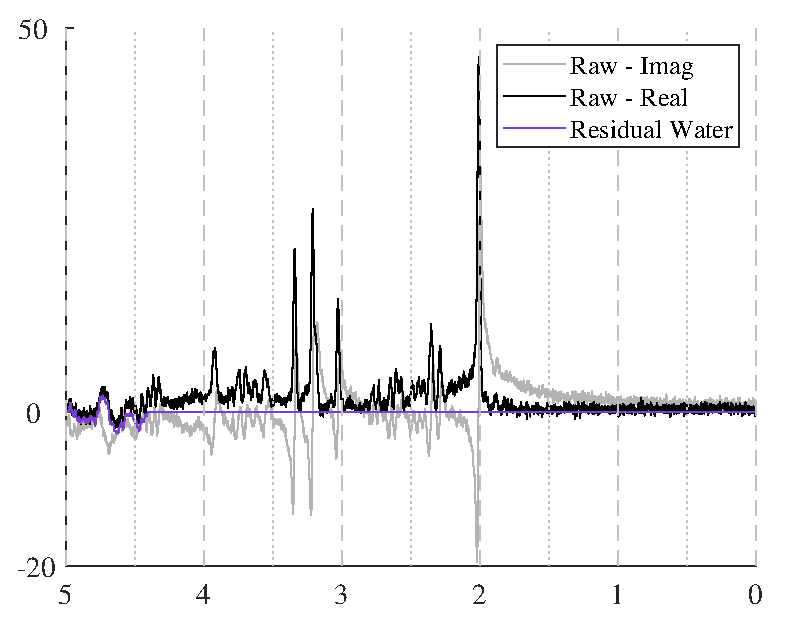
\includegraphics[width=0.93\textwidth]{images/samples_by_artifact/30ms_artifact_samples_voigt_1.eps}
    %     \caption{${T_2}^* \times 0.10$ and $G=20$Hz}
    %     \vspace{3pt}
    % \end{subfigure}&
    % \begin{subfigure}[c]{0.31\textwidth}
    %     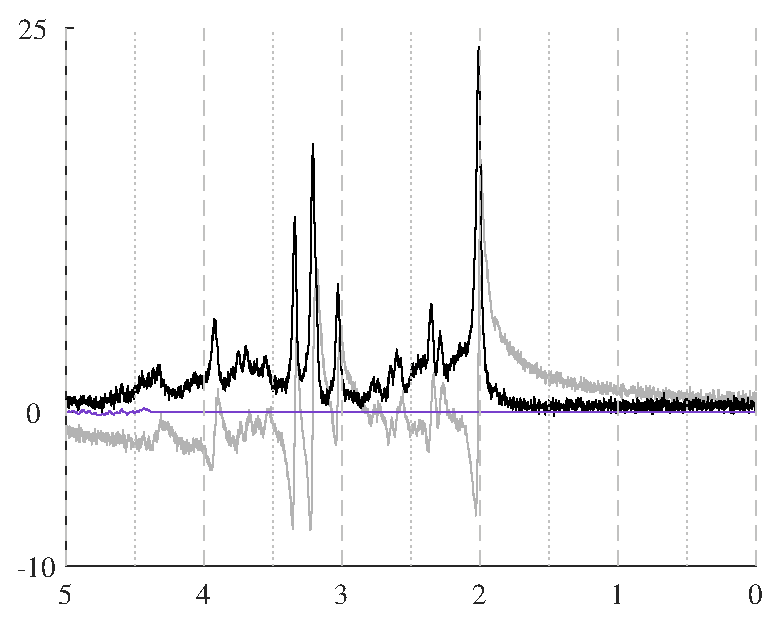
\includegraphics[width=0.93\textwidth]{images/samples_by_artifact/30ms_artifact_samples_voigt_2.eps}
    %     \caption{${T_2}^* \times 1.00$ and $G=20$Hz}
    %     \vspace{3pt}
    % \end{subfigure}&
    % \begin{subfigure}[c]{0.31\textwidth}
    %     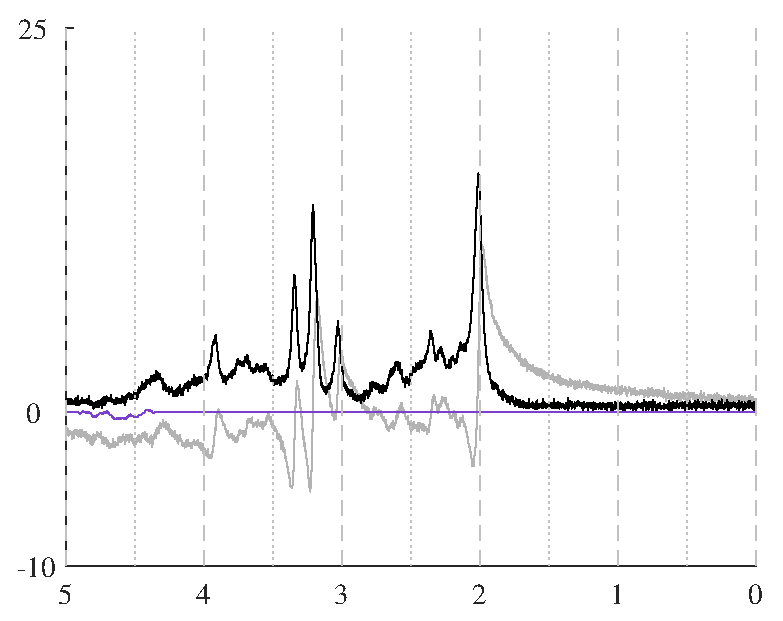
\includegraphics[width=0.93\textwidth]{images/samples_by_artifact/30ms_artifact_samples_voigt_3.eps}
    %     \caption{${T_2}^* \times 2.00$ and $G=20$Hz}
    %     \vspace{3pt}
    % \end{subfigure}\\
    % \begin{subfigure}[c]{0.31\textwidth}
    %     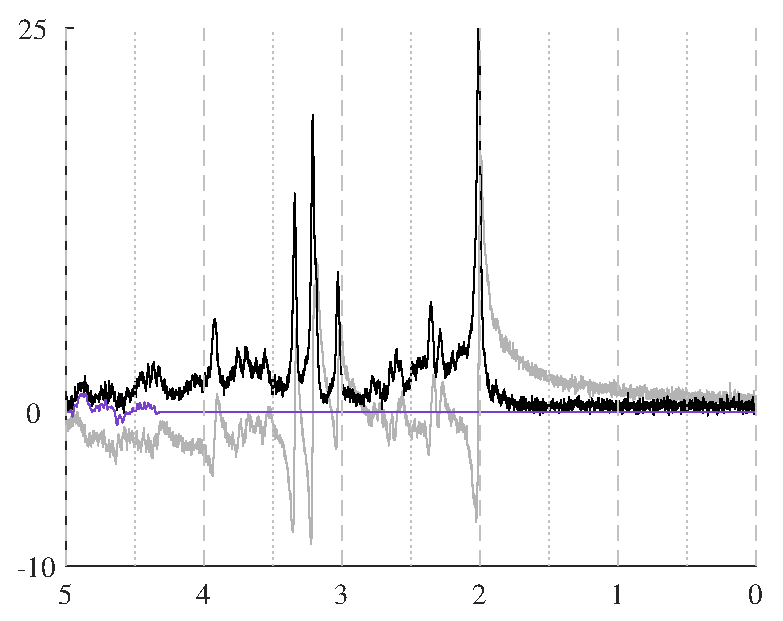
\includegraphics[width=0.93\textwidth]{images/samples_by_artifact/30ms_artifact_samples_voigt_4.eps}
    %     \caption{${T_2}^* \times 1.00$ and $G=10$Hz}
    %     \vspace{3pt}
    % \end{subfigure}&
    % \begin{subfigure}[c]{0.31\textwidth}
    %     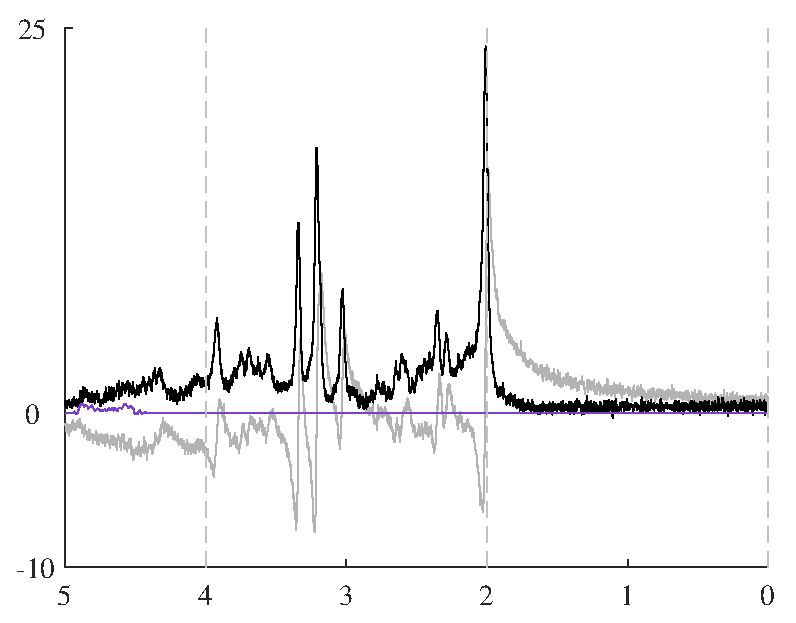
\includegraphics[width=0.93\textwidth]{images/samples_by_artifact/30ms_artifact_samples_voigt_5.eps}
    %     \caption{${T_2}^* \times 1.00$ and $G=20$Hz}
    %     \vspace{3pt}
    % \end{subfigure}&%
    % \begin{subfigure}[c]{0.31\textwidth}
    %     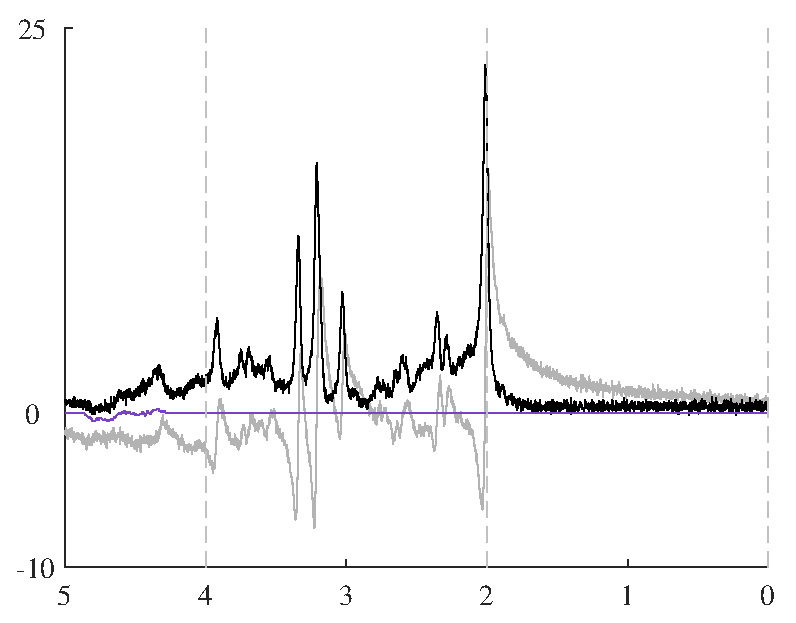
\includegraphics[width=0.93\textwidth]{images/samples_by_artifact/30ms_artifact_samples_voigt_6.eps}
    %     \caption{${T_2}^* \times 1.00$ and $G=30$Hz}
    %     \vspace{3pt}
    % \end{subfigure}\\
    % \end{tabular}
    \includegraphics[width=\textwidth,keepaspectratio]{images/compiled_figures/MRS_Sim_Figure_10_Voigt_Broadening_samples.png}
    \caption{Theses samples explore the effects of lorentzian and gaussian broadening on the Voigt lineshape. The spectral SNR = 15. No phase offsets, eddy currents, or baselines were included. The top row varies the lorentzian broadening with a fixed gaussian value where the bottom row fixes the lorentzian broadening values and varies the gaussian.}
    \label{fig:30ms samples voigt}
\end{figure}


% \begin{figure}[ht!]
    \centering
    % \begin{tabular}[c]{ccc}
    % \begin{subfigure}[c]{0.31\textwidth}
    %     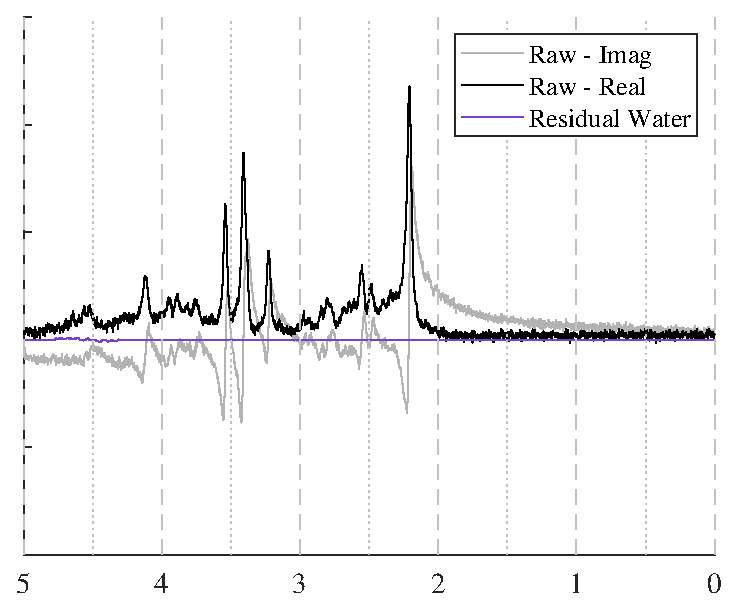
\includegraphics[width=0.93\textwidth]{images/samples_by_artifact/30ms_artifact_samples_fshift_1.eps}
    %     \caption{F\textsubscript{shift} = 0.2 ppm = 160 Hz}
    %     \vspace{3pt}
    % \end{subfigure}&
    % \begin{subfigure}[c]{0.31\textwidth}
    %     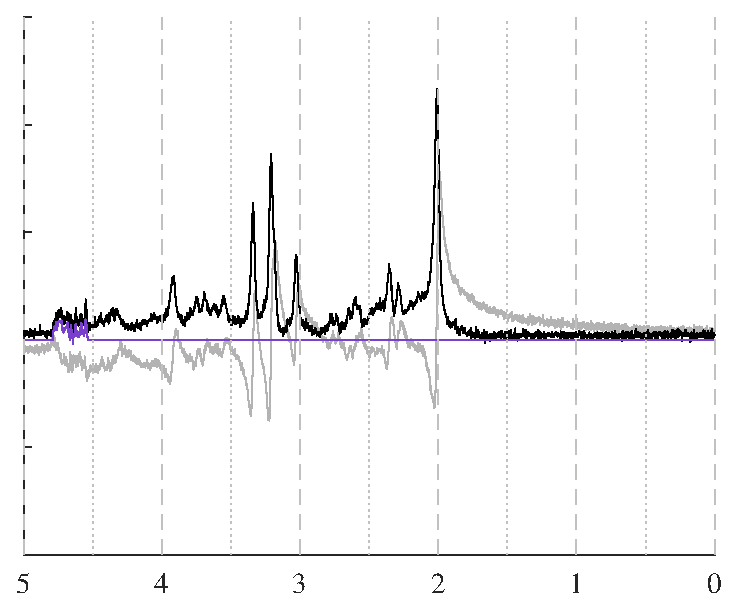
\includegraphics[width=0.93\textwidth]{images/samples_by_artifact/30ms_artifact_samples_fshift_2.eps}
    %     \caption{F\textsubscript{shift} = 0.0 ppm = 0 Hz}
    %     \vspace{3pt}
    % \end{subfigure}&
    % \begin{subfigure}[c]{0.31\textwidth}
    %     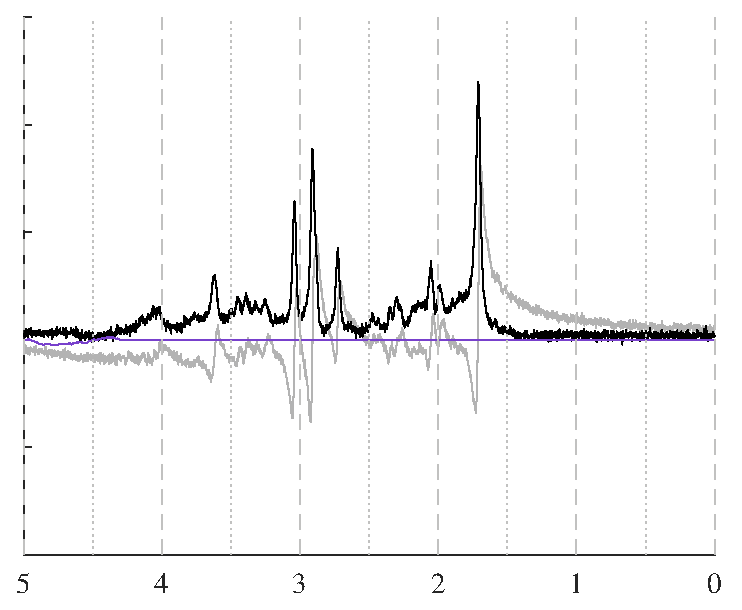
\includegraphics[width=0.93\textwidth]{images/samples_by_artifact/30ms_artifact_samples_fshift_3.eps}
    %     \caption{F\textsubscript{shift} = -0.3 ppm = -240 Hz}
    %     \vspace{3pt}
    % \end{subfigure}\\
    % \begin{subfigure}[c]{0.31\textwidth}
    %     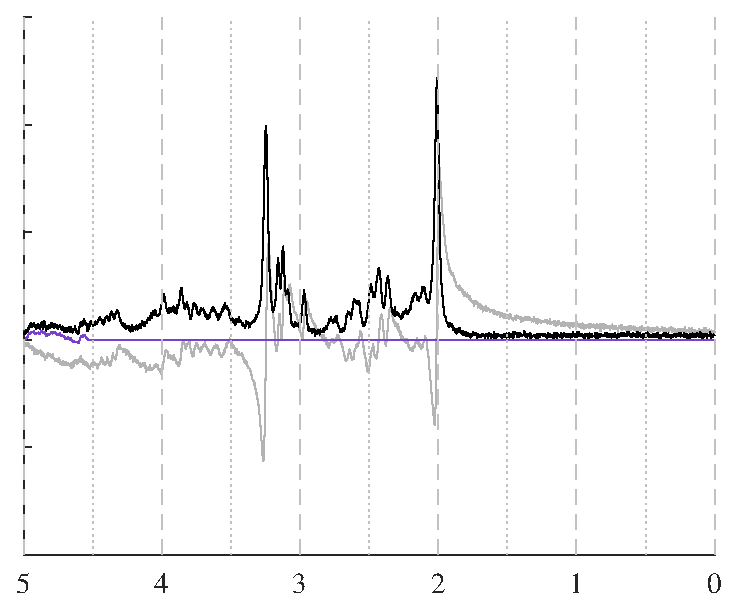
\includegraphics[width=0.93\textwidth]{images/samples_by_artifact/30ms_artifact_samples_fshift_4.eps}
    %     \caption{F\textsubscript{shift} $\in [-0.10, 0.10]$ ppm = $\pm 80$Hz}
    %     \vspace{3pt}
    % \end{subfigure}&
    % \begin{subfigure}[c]{0.31\textwidth}
    %     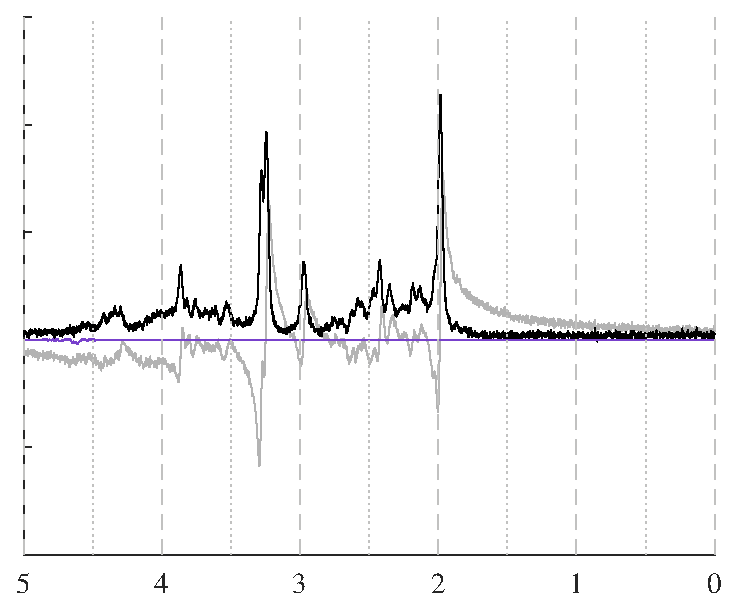
\includegraphics[width=0.93\textwidth]{images/samples_by_artifact/30ms_artifact_samples_fshift_5.eps}
    %     \caption{F\textsubscript{shift} $\in [-0.10, 0.10]$ ppm = $\pm 80$Hz}
    %     \vspace{3pt}
    % \end{subfigure}&%
    % \begin{subfigure}[c]{0.31\textwidth}
    %     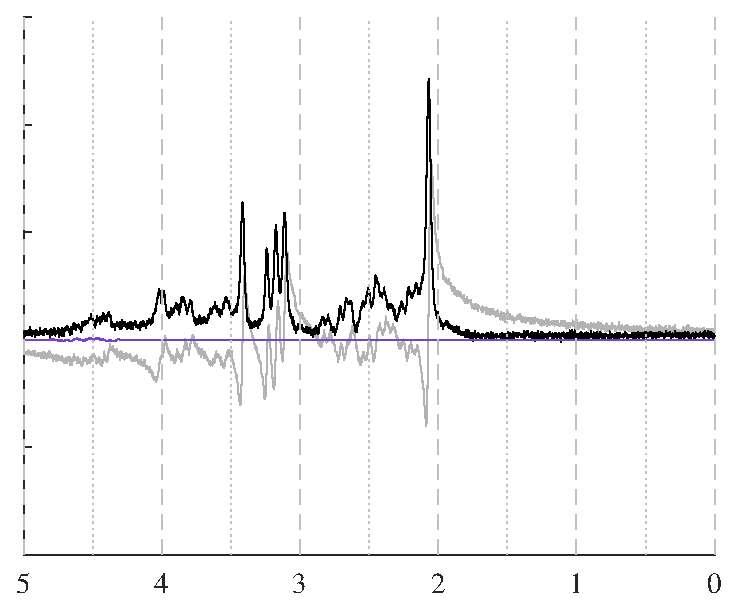
\includegraphics[width=0.93\textwidth]{images/samples_by_artifact/30ms_artifact_samples_fshift_6.eps}
    %     \caption{F\textsubscript{shift} $\in [-0.10, 0.10]$ ppm = $\pm 80$Hz}
    %     \vspace{3pt}
    % \end{subfigure}\\
    % \end{tabular}
    \includegraphics[width=\textwidth,keepaspectratio]{images/compiled_figures/MRS_Sim_Figure_11_Frequency_Shifts_samples.png}
    \caption{Two types of frequency shifts are shown in these examples. The top row shows global frequency shifts. The bottom row shows the effects of using randomly sampled metabolite-level frequency shifts. The spectral SNR = 15 with fixed lorentzian and gaussian broadening. No baselines, phase offsets, or eddy currents were included.}
    \label{fig:30ms samples fshift}
\end{figure}


% \begin{figure}[ht!]
    \centering
    % \begin{tabular}[c]{ccc}
    % \begin{subfigure}[c]{0.31\textwidth}
    %     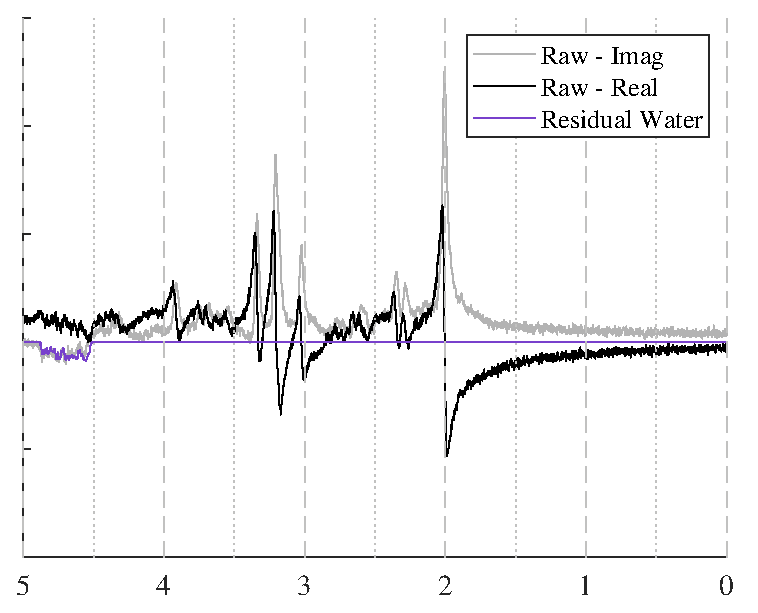
\includegraphics[width=0.93\textwidth]{images/samples_by_artifact/30ms_artifact_samples_phi0_1.eps}
    %     \caption{$\Phi_0 = -64^\circ$}
    %     \vspace{3pt}
    % \end{subfigure}&
    % \begin{subfigure}[c]{0.31\textwidth}
    %     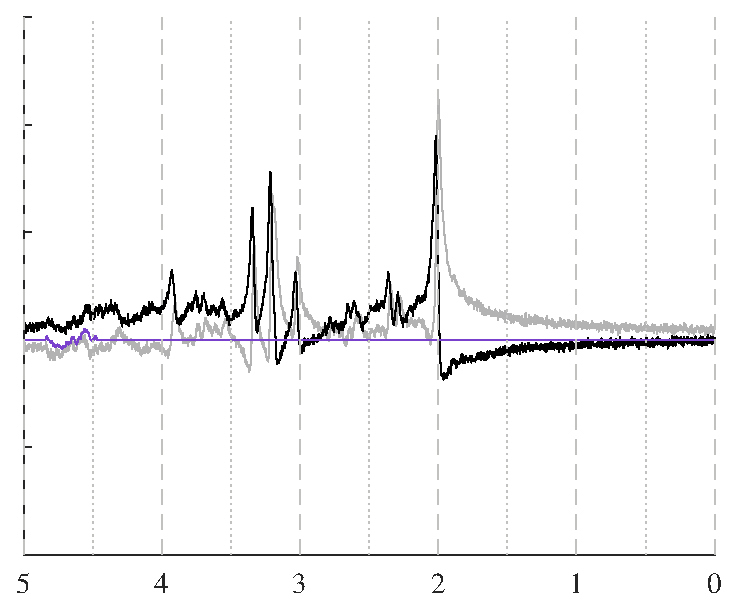
\includegraphics[width=0.93\textwidth]{images/samples_by_artifact/30ms_artifact_samples_phi0_2.eps}
    %     \caption{$\Phi_0 = -35^\circ$}
    %     \vspace{3pt}
    % \end{subfigure}&
    % \begin{subfigure}[c]{0.31\textwidth}
    %     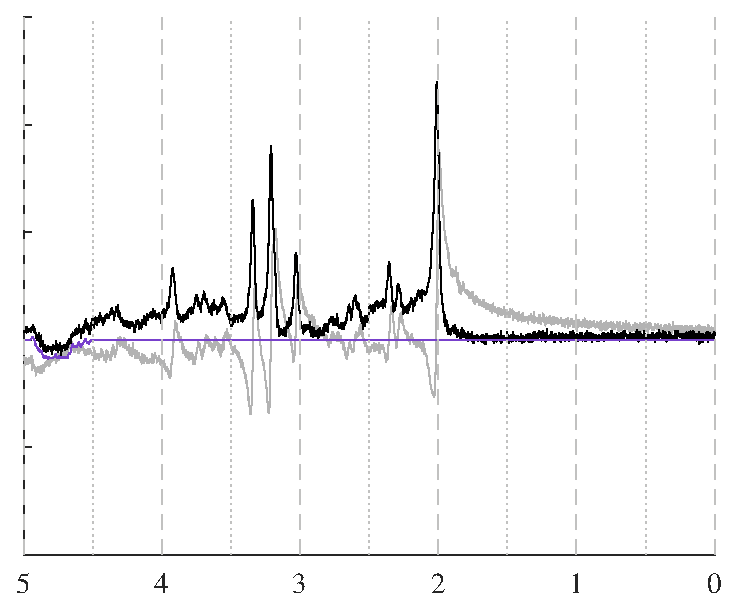
\includegraphics[width=0.93\textwidth]{images/samples_by_artifact/30ms_artifact_samples_phi0_3.eps}
    %     \caption{$\Phi_0 = -5^\circ$}
    %     \vspace{3pt}
    % \end{subfigure}\\
    % \begin{subfigure}[c]{0.31\textwidth}
    %     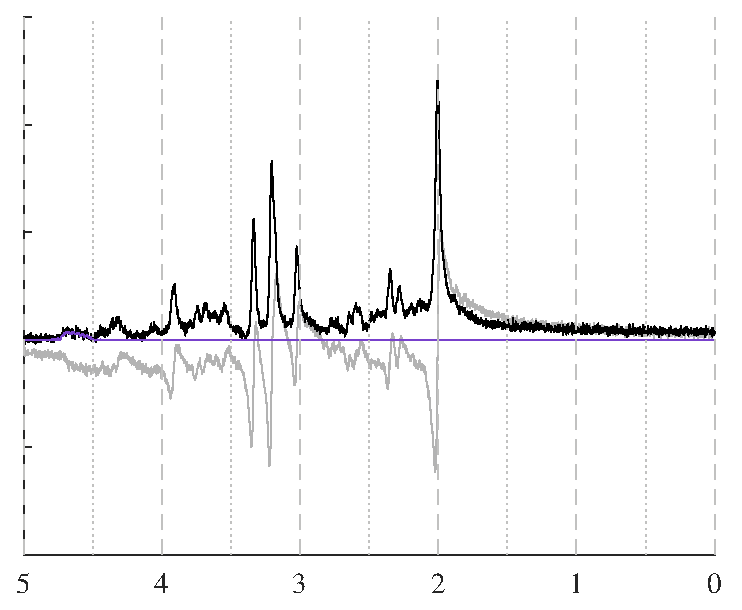
\includegraphics[width=0.93\textwidth]{images/samples_by_artifact/30ms_artifact_samples_phi0_4.eps}
    %     \caption{$\Phi_0 = 25^\circ$}
    %     \vspace{3pt}
    % \end{subfigure}&
    % \begin{subfigure}[c]{0.31\textwidth}
    %     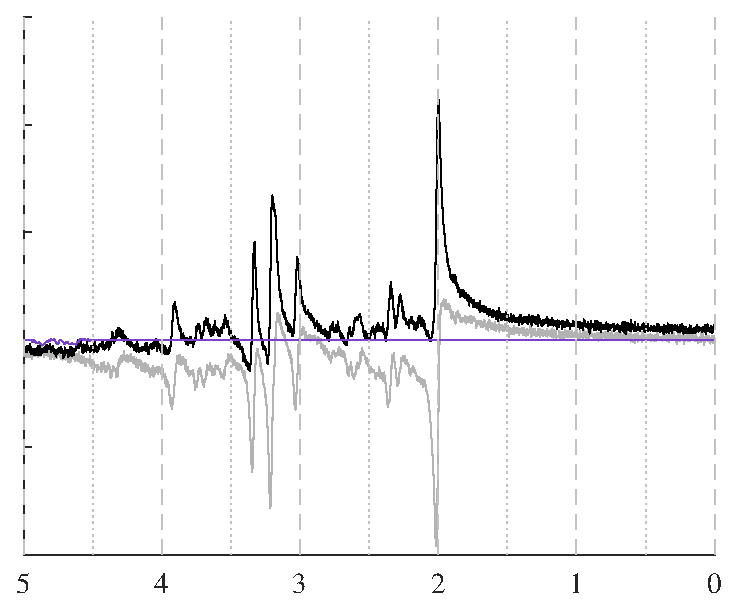
\includegraphics[width=0.93\textwidth]{images/samples_by_artifact/30ms_artifact_samples_phi0_5.eps}
    %     \caption{$\Phi_0 = 55^\circ$}
    %     \vspace{3pt}
    % \end{subfigure}&%
    % \begin{subfigure}[c]{0.31\textwidth}
    %     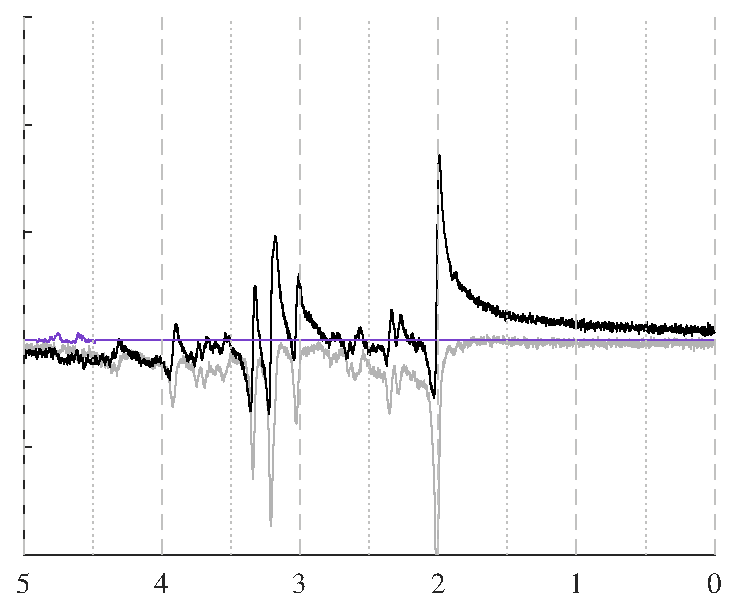
\includegraphics[width=0.93\textwidth]{images/samples_by_artifact/30ms_artifact_samples_phi0_6.eps}
    %     \caption{$\Phi_0 = 85^\circ$}
    %     \vspace{3pt}
    % \end{subfigure}\\
    % \end{tabular}
    \includegraphics[width=\textwidth,keepaspectratio]{images/compiled_figures/MRS_Sim_Figure_12_Zero-Order_Phase_samples.png}
    \caption{Identical spectra are displayed with varying zero-order phase offsets as indicated below each plot. The lorentzian broadening was left unscaled, gaussian broadening = 20 Hz, spectral SNR = 15. First-order phase and eddy currents were omitted.}
    \label{fig:30ms samples phi0}
\end{figure}


% \begin{figure}[ht!]
    \centering
    % \begin{tabular}[c]{ccc}
    % \begin{subfigure}[c]{0.31\textwidth}
    %     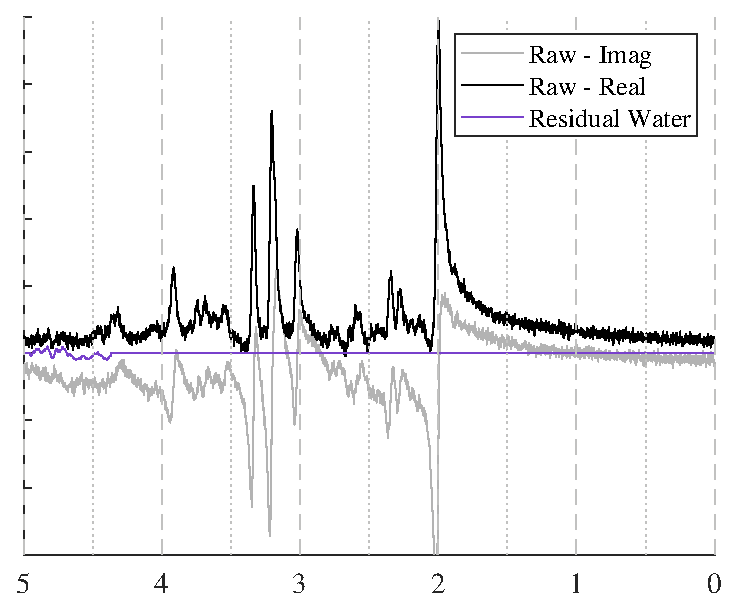
\includegraphics[width=0.93\textwidth]{images/samples_by_artifact/30ms_artifact_samples_phi1_1.eps}
    %     \caption{$\Phi_1 = -20^\circ$}
    %     \vspace{3pt}
    % \end{subfigure}&
    % \begin{subfigure}[c]{0.31\textwidth}
    %     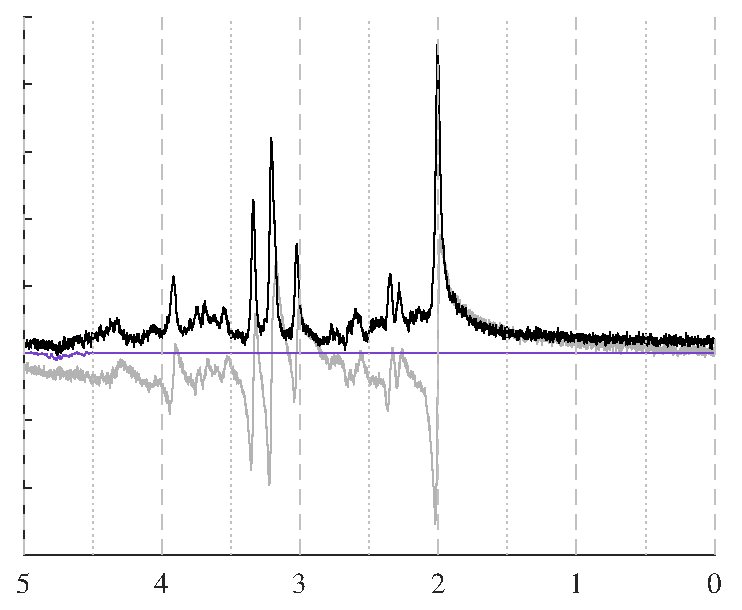
\includegraphics[width=0.93\textwidth]{images/samples_by_artifact/30ms_artifact_samples_phi1_2.eps}
    %     \caption{$\Phi_1 = -11^\circ$}
    %     \vspace{3pt}
    % \end{subfigure}&
    % \begin{subfigure}[c]{0.31\textwidth}
    %     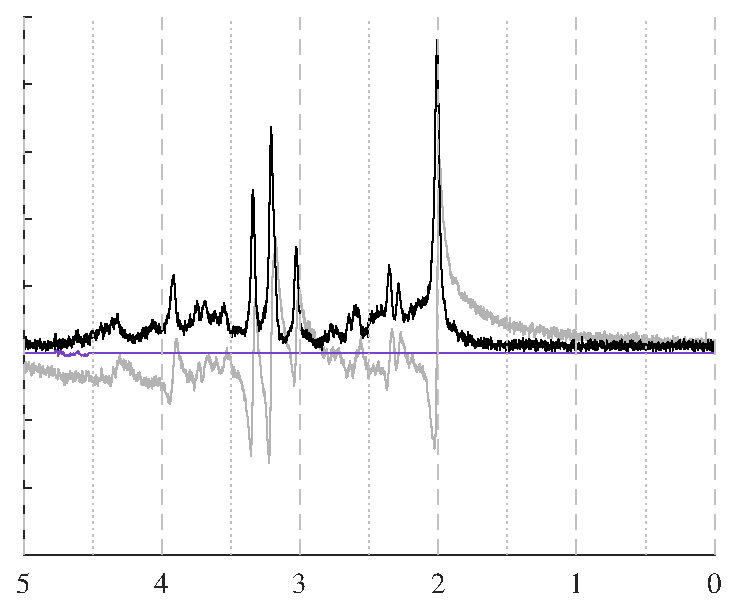
\includegraphics[width=0.93\textwidth]{images/samples_by_artifact/30ms_artifact_samples_phi1_3.eps}
    %     \caption{$\Phi_1 = -2^\circ$}
    %     \vspace{3pt}
    % \end{subfigure}\\
    % \begin{subfigure}[c]{0.31\textwidth}
    %     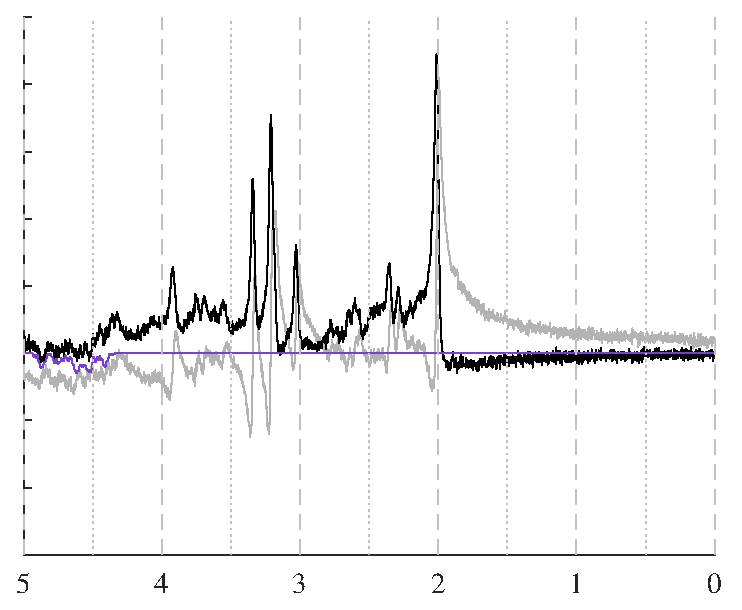
\includegraphics[width=0.93\textwidth]{images/samples_by_artifact/30ms_artifact_samples_phi1_4.eps}
    %     \caption{$\Phi_1 = 7^\circ$}
    %     \vspace{3pt}
    % \end{subfigure}&
    % \begin{subfigure}[c]{0.31\textwidth}
    %     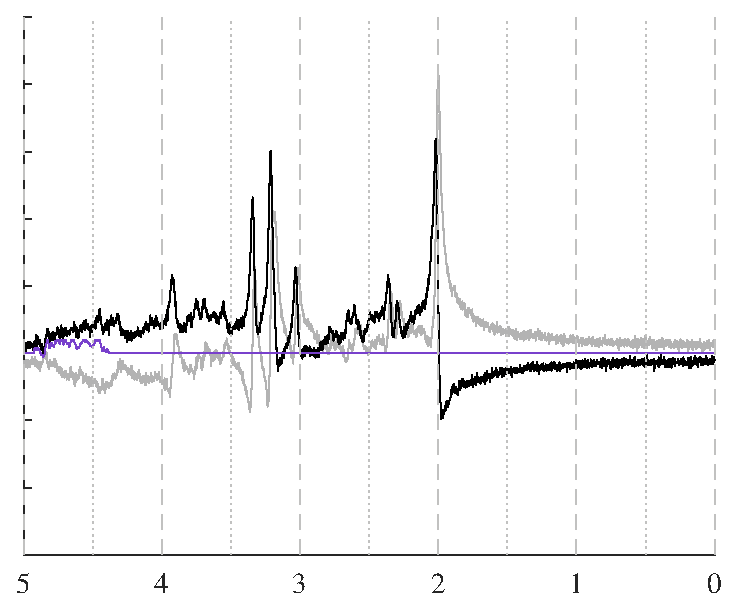
\includegraphics[width=0.93\textwidth]{images/samples_by_artifact/30ms_artifact_samples_phi1_5.eps}
    %     \caption{$\Phi_1 = 16^\circ$}
    %     \vspace{3pt}
    % \end{subfigure}&%
    % \begin{subfigure}[c]{0.31\textwidth}
    %     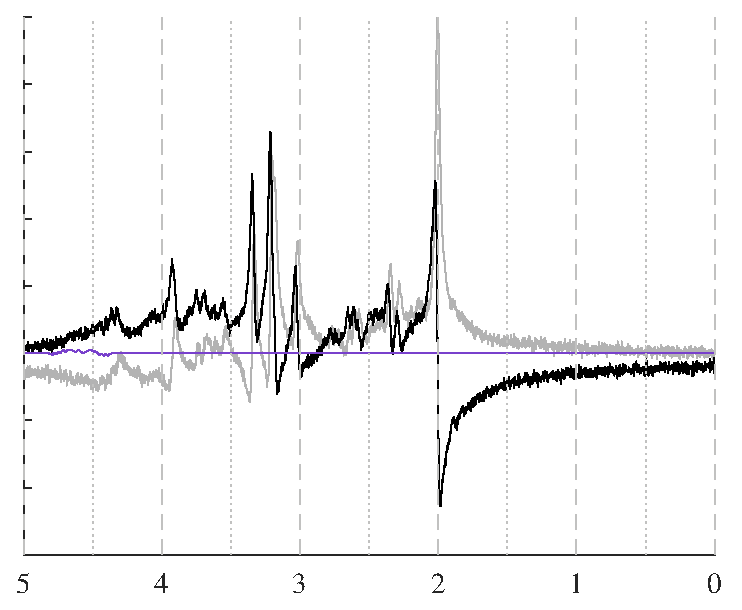
\includegraphics[width=0.93\textwidth]{images/samples_by_artifact/30ms_artifact_samples_phi1_6.eps}
    %     \caption{$\Phi_1 = 25^\circ$}
    %     \vspace{3pt}
    % \end{subfigure}\\
    % \end{tabular}
    \includegraphics[width=\textwidth,keepaspectratio]{images/compiled_figures/MRS_Sim_Figure_13_First-Order_Phase_samples.png}
    \caption{Identical spectra are displayed with varying first-order phase offsets as indicated below each plot. The lorentzian broadening was left unscaled. The gaussian broadening = 20 Hz and the spectral SNR = 15. Zero-order phase, and eddy currents were omitted.}
    \label{fig:30ms samples phi1}
\end{figure}


% \begin{figure}[ht!]
    \centering
    % \begin{tabular}[c]{ccc}
    % \begin{subfigure}[c]{0.31\textwidth}
    %     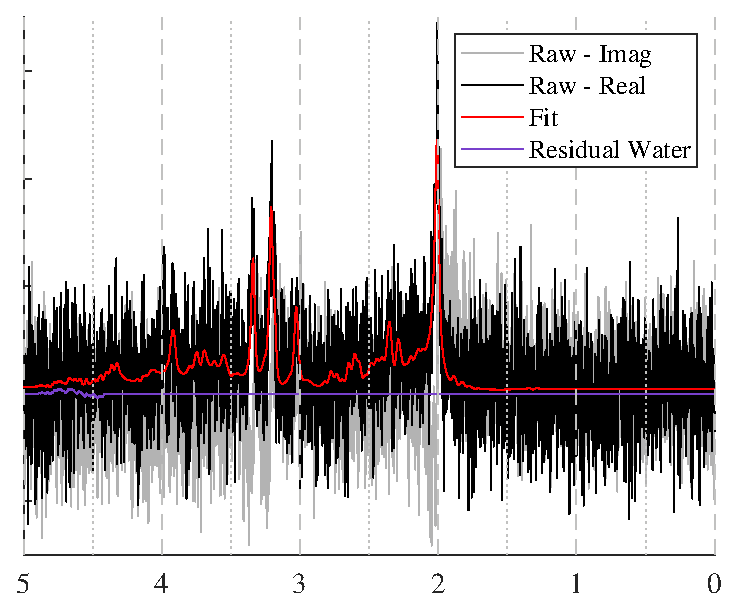
\includegraphics[width=0.93\textwidth]{images/samples_by_artifact/30ms_artifact_samples_snr_1.eps}
    %     \caption{Spectral SNR=2}
    %     \vspace{3pt}
    % \end{subfigure}&
    % \begin{subfigure}[c]{0.31\textwidth}
    %     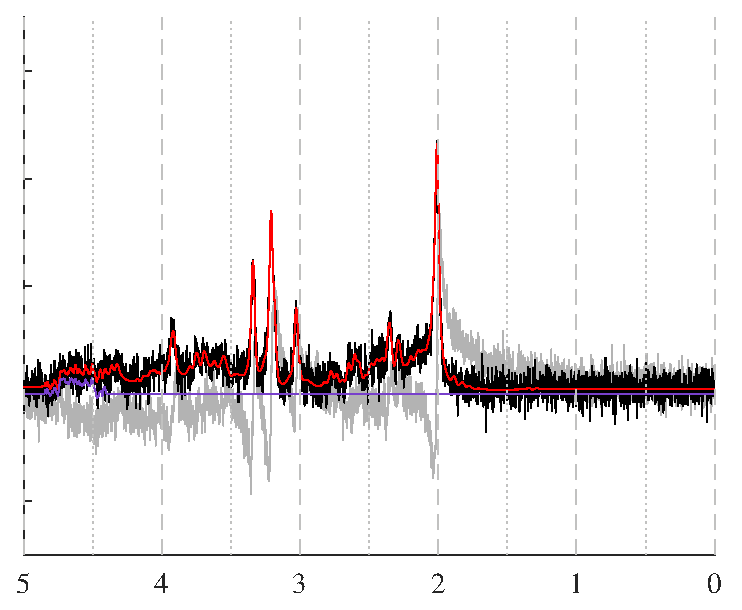
\includegraphics[width=0.93\textwidth]{images/samples_by_artifact/30ms_artifact_samples_snr_2.eps}
    %     \caption{Spectral SNR=8}
    %     \vspace{3pt}
    % \end{subfigure}&
    % \begin{subfigure}[c]{0.31\textwidth}
    %     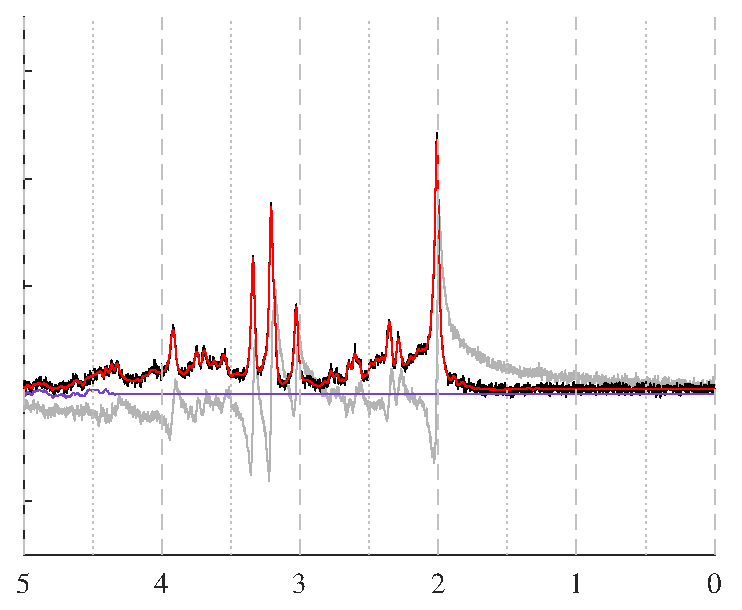
\includegraphics[width=0.93\textwidth]{images/samples_by_artifact/30ms_artifact_samples_snr_3.eps}
    %     \caption{Spectral SNR=14}
    %     \vspace{3pt}
    % \end{subfigure}\\
    % \begin{subfigure}[c]{0.31\textwidth}
    %     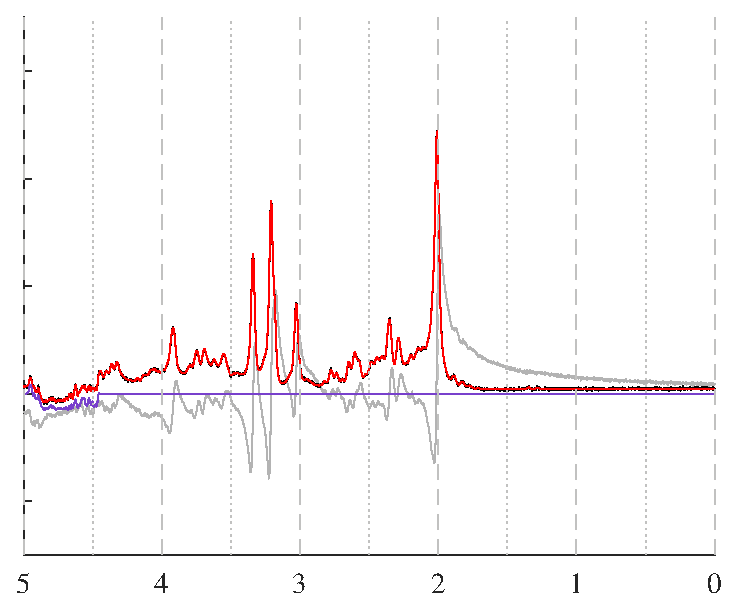
\includegraphics[width=0.93\textwidth]{images/samples_by_artifact/30ms_artifact_samples_snr_4.eps}
    %     \caption{Spectral SNR=20}
    %     \vspace{3pt}
    % \end{subfigure}&
    % \begin{subfigure}[c]{0.31\textwidth}
    %     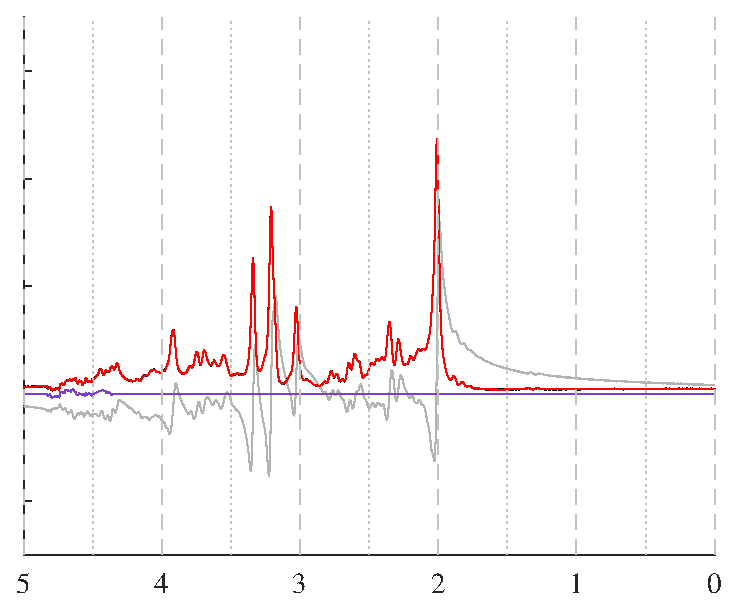
\includegraphics[width=0.93\textwidth]{images/samples_by_artifact/30ms_artifact_samples_snr_5.eps}
    %     \caption{Spectral SNR=26}
    %     \vspace{3pt}
    % \end{subfigure}&%
    % \begin{subfigure}[c]{0.31\textwidth}
    %     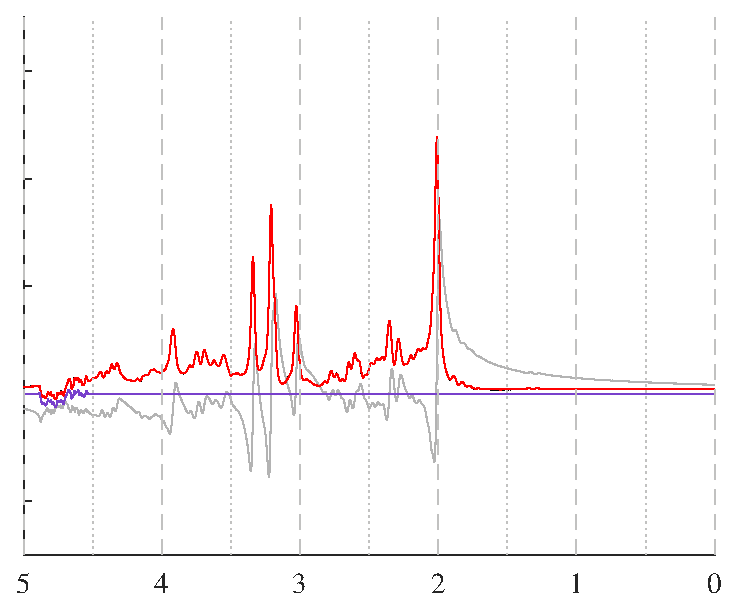
\includegraphics[width=0.93\textwidth]{images/samples_by_artifact/30ms_artifact_samples_snr_6.eps}
    %     \caption{Spectral SNR=32}
    %     \vspace{3pt}
    % \end{subfigure}\\
    % \end{tabular}
    \includegraphics[width=\textwidth,keepaspectratio]{images/compiled_figures/MRS_Sim_Figure_14_SNR_samples.png}
    \caption{Identical spectra are displayed with varying spectral SNRs as indicated below each plot. The lorentzian broadening was left unscaled and the gaussian broadening = 20 Hz. All phase offsets and eddy currents were omitted.}
    \label{fig:30ms samples snr}
\end{figure}


% \begin{figure}[t!]
    \centering
    % \begin{tabular}[c]{ccc}
    % \begin{subfigure}[c]{0.31\textwidth}
    %     \includegraphics[width=0.93\textwidth]{images/samples_by_artifact/30ms_artifact_samples_ecc_1.eps}
    %     \caption{$A=1.0$ Hz, $t_c=0.15$ s}
    %     \vspace{3pt}
    % \end{subfigure}&
    % \begin{subfigure}[c]{0.31\textwidth}
    %     \includegraphics[width=0.93\textwidth]{images/samples_by_artifact/30ms_artifact_samples_ecc_2.eps}
    %     \caption{$A=5.5$ Hz, $t_c=0.15$ s}
    %     \vspace{3pt}
    % \end{subfigure}&
    % \begin{subfigure}[c]{0.31\textwidth}
    %     \includegraphics[width=0.93\textwidth]{images/samples_by_artifact/30ms_artifact_samples_ecc_3.eps}
    %     \caption{$A=10.0$ Hz, $t_c=0.15$ s}
    %     \vspace{3pt}
    % \end{subfigure}\\
    % \begin{subfigure}[c]{0.31\textwidth}
    %     \includegraphics[width=0.93\textwidth]{images/samples_by_artifact/30ms_artifact_samples_ecc_4.eps}
    %     \caption{$A=5.0$ Hz, $t_c=0.02$ s}
    %     % \vspace{3pt}
    % \end{subfigure}&
    % \begin{subfigure}[c]{0.31\textwidth}
    %     \includegraphics[width=0.93\textwidth]{images/samples_by_artifact/30ms_artifact_samples_ecc_5.eps}
    %     \caption{$A=5.0$ Hz, $t_c=0.16$ s}
    %     % \vspace{3pt}
    % \end{subfigure}&%
    % \begin{subfigure}[c]{0.31\textwidth}
    %     \includegraphics[width=0.93\textwidth]{images/samples_by_artifact/30ms_artifact_samples_ecc_6.eps}
    %     \caption{$A=5.0$ Hz, $t_c=0.30$ s}
    %     % \vspace{3pt}
    % \end{subfigure}\\
    % \end{tabular}
    \includegraphics[width=0.95\textwidth,keepaspectratio]{images/compiled_figures/MRS_Sim_Figure_15_ECC_samples.png}
    \caption{Eddy currents are simulated with two variables: an amplitude, A, and a time constant, $t_c$. In the top row, $t_c$ is fixed to 0.15 seconds and the amplitudes are set to 1Hz, 5.5Hz, and 10Hz. In the bottom row, the amplitude is fixed to 5Hz and the time constants are set to 0.02 sec, 0.16 sec, and 0.30 sec. The values listed correspond to the plots from left to right.}
    \label{fig:30ms samples ecc}
\end{figure}



% The following collection of figures show the effects of several standard spectral model components when their parameters are varied. These examples use the same spectrum which was simulated using the following basis functions with fixed concentrations for all simulations: Asc, Asp, Ch, Cr, GABA, GPC, GSH, Gln, Glu, mI, Lac, NAA, NAAG, PCh, PCr, PE, sI, Tau, MM09, MM12, MM14, MM17, MM20, Lip09, Lip13, and Lip20. Standard T2 values were assigned to each based on values present by Wyss et al.\cite{Wyss2018}. When spectral components are not being studied, their values are fixed. Baselines were omitted to better highlight the impact of the individual components.

The following collection of figures show the effects of several standard spectral model components when their parameters are varied. When spectral components are not being studied, their values are fixed. Fig. \ref{fig:30ms samples lorentzians} shows the effect of lorentzian line broadening in the absence of any gaussian broadening. In the top row, the height of the y-axis drops from left-to-right showing the decrease in signal intensity. On the bottom row the differences are not as severe, so a single y-axis is used. Here it is more clearly shown that the spectral peaks are both losing intensity %\FloatBarrier 
% \noindent 
and widening. Fig. \ref{fig:30ms samples gaussians} uses the same display protocol to show the effects of gaussian broadening without lorentzian broadening whereas Fig. \ref{fig:30ms samples voigt} shows several combinations of lorentzian and gaussian broadening that, when combined, give the Voigt lineshape. Fig. \ref{fig:30ms samples voigt} breaks down the effects of the lorentzian and gaussian broadening on the Voigt lineshape in the top and bottom rows. On top, the gaussian value is fixed to 20Hz while scaling the $T_2^*$ values using the scaling factors indicated in the captions. On the bottom, the lorentzian broadening is fixed and the gaussian values vary.

\begin{figure}[b!]
    \centering
    % \begin{tabular}[c]{ccc}
    % \begin{subfigure}[c]{0.31\textwidth}
    %     \includegraphics[width=0.93\textwidth]{images/samples_by_artifact/30ms_artifact_samples_lorentzian_1.eps}
    %     \caption{${T_2}^* \times 0.25$}
    %     \vspace{3pt}
    % \end{subfigure}&
    % \begin{subfigure}[c]{0.31\textwidth}
    %     \includegraphics[width=0.93\textwidth]{images/samples_by_artifact/30ms_artifact_samples_lorentzian_2.eps}
    %     \caption{${T_2}^* \times 0.50$}
    %     \vspace{3pt}
    % \end{subfigure}&
    % \begin{subfigure}[c]{0.31\textwidth}
    %     \includegraphics[width=0.93\textwidth]{images/samples_by_artifact/30ms_artifact_samples_lorentzian_3.eps}
    %     \caption{${T_2}^* \times 0.75$}
    %     \vspace{3pt}
    % \end{subfigure}\\
    % \begin{subfigure}[c]{0.31\textwidth}
    %     \includegraphics[width=0.93\textwidth]{images/samples_by_artifact/30ms_artifact_samples_lorentzian_4.eps}
    %     \caption{${T_2}^* \times 1.00$}
    %     \vspace{3pt}
    % \end{subfigure}&
    % \begin{subfigure}[c]{0.31\textwidth}
    %     \includegraphics[width=0.93\textwidth]{images/samples_by_artifact/30ms_artifact_samples_lorentzian_5.eps}
    %     \caption{${T_2}^* \times 1.25$}
    %     \vspace{3pt}
    % \end{subfigure}&%
    % \begin{subfigure}[c]{0.31\textwidth}
    %     \includegraphics[width=0.93\textwidth]{images/samples_by_artifact/30ms_artifact_samples_lorentzian_6.eps}
    %     \caption{${T_2}^* \times 1.50$}
    %     \vspace{3pt}
    % \end{subfigure}\\
    % \end{tabular}
    \includegraphics[width=\textwidth,keepaspectratio]{images/compiled_figures/MRS_Sim_Figure_8_Lorentzian_Broadening_samples.png}
    \caption{${T_2}^*$ values were fixed and then scaled to represent varying magnitudes of lorentzian broadening. The spectral SNR = 15. No gaussian broadening, baselines, phase offsets, or eddy currents were included.}
    \label{fig:30ms samples lorentzians}
\end{figure}


\begin{figure}[ht!]
    \centering
    % \begin{tabular}[c]{ccc}
    % \begin{subfigure}[c]{0.31\textwidth}
    %     \includegraphics[width=0.93\textwidth]{images/samples_by_artifact/30ms_artifact_samples_gaussian_1.eps}
    %     \caption{Gaussian = 1.0 Hz}
    %     \vspace{3pt}
    % \end{subfigure}&
    % \begin{subfigure}[c]{0.31\textwidth}
    %     \includegraphics[width=0.93\textwidth]{images/samples_by_artifact/30ms_artifact_samples_gaussian_2.eps}
    %     \caption{Gaussian = 14.9 Hz}
    %     \vspace{3pt}
    % \end{subfigure}&
    % \begin{subfigure}[c]{0.31\textwidth}
    %     \includegraphics[width=0.93\textwidth]{images/samples_by_artifact/30ms_artifact_samples_gaussian_3.eps}
    %     \caption{Gaussian = 28.8 Hz}
    %     \vspace{3pt}
    % \end{subfigure}\\
    % \begin{subfigure}[c]{0.31\textwidth}
    %     \includegraphics[width=0.93\textwidth]{images/samples_by_artifact/30ms_artifact_samples_gaussian_4.eps}
    %     \caption{Gaussian = 42.8 Hz}
    %     \vspace{3pt}
    % \end{subfigure}&
    % \begin{subfigure}[c]{0.31\textwidth}
    %     \includegraphics[width=0.93\textwidth]{images/samples_by_artifact/30ms_artifact_samples_gaussian_5.eps}
    %     \caption{Gaussian = 56.7 Hz}
    %     \vspace{3pt}
    % \end{subfigure}&%
    % \begin{subfigure}[c]{0.31\textwidth}
    %     \includegraphics[width=0.93\textwidth]{images/samples_by_artifact/30ms_artifact_samples_gaussian_6.eps}
    %     \caption{Gaussian = 70.7 Hz}
    %     \vspace{3pt}
    % \end{subfigure}\\
    % \end{tabular}
    \includegraphics[width=\textwidth,keepaspectratio]{images/compiled_figures/MRS_Sim_Figure_9_Gaussian_Broadening_samples.png}
    \caption{Gaussian broadening values were sampled from [0,70.17] in increasing order, as displayed beneath each plot. The lorentzian broadening was left unscaled (scaling coeffient = 1.0 corresponding to Fig. \ref{fig:30ms samples lorentzians}). The spectral SNR = 15 and phase offsets and eddy currents were omitted.}
    \label{fig:30ms samples gaussians}
\end{figure}


\begin{figure}[ht!]
    \centering
    % % \includegraphics[width=\textwidth,keepaspectratio]{images/compiled_figures/MRS_Sim_Figure_10_Voigt_Broadening_samples.eps}
    % \begin{tabular}[c]{ccc}
    % \begin{subfigure}[c]{0.31\textwidth}
    %     \includegraphics[width=0.93\textwidth]{images/samples_by_artifact/30ms_artifact_samples_voigt_1.eps}
    %     \caption{${T_2}^* \times 0.10$ and $G=20$Hz}
    %     \vspace{3pt}
    % \end{subfigure}&
    % \begin{subfigure}[c]{0.31\textwidth}
    %     \includegraphics[width=0.93\textwidth]{images/samples_by_artifact/30ms_artifact_samples_voigt_2.eps}
    %     \caption{${T_2}^* \times 1.00$ and $G=20$Hz}
    %     \vspace{3pt}
    % \end{subfigure}&
    % \begin{subfigure}[c]{0.31\textwidth}
    %     \includegraphics[width=0.93\textwidth]{images/samples_by_artifact/30ms_artifact_samples_voigt_3.eps}
    %     \caption{${T_2}^* \times 2.00$ and $G=20$Hz}
    %     \vspace{3pt}
    % \end{subfigure}\\
    % \begin{subfigure}[c]{0.31\textwidth}
    %     \includegraphics[width=0.93\textwidth]{images/samples_by_artifact/30ms_artifact_samples_voigt_4.eps}
    %     \caption{${T_2}^* \times 1.00$ and $G=10$Hz}
    %     \vspace{3pt}
    % \end{subfigure}&
    % \begin{subfigure}[c]{0.31\textwidth}
    %     \includegraphics[width=0.93\textwidth]{images/samples_by_artifact/30ms_artifact_samples_voigt_5.eps}
    %     \caption{${T_2}^* \times 1.00$ and $G=20$Hz}
    %     \vspace{3pt}
    % \end{subfigure}&%
    % \begin{subfigure}[c]{0.31\textwidth}
    %     \includegraphics[width=0.93\textwidth]{images/samples_by_artifact/30ms_artifact_samples_voigt_6.eps}
    %     \caption{${T_2}^* \times 1.00$ and $G=30$Hz}
    %     \vspace{3pt}
    % \end{subfigure}\\
    % \end{tabular}
    \includegraphics[width=\textwidth,keepaspectratio]{images/compiled_figures/MRS_Sim_Figure_10_Voigt_Broadening_samples.png}
    \caption{Theses samples explore the effects of lorentzian and gaussian broadening on the Voigt lineshape. The spectral SNR = 15. No phase offsets, eddy currents, or baselines were included. The top row varies the lorentzian broadening with a fixed gaussian value where the bottom row fixes the lorentzian broadening values and varies the gaussian.}
    \label{fig:30ms samples voigt}
\end{figure}


\begin{figure}[ht!]
    \centering
    % \begin{tabular}[c]{ccc}
    % \begin{subfigure}[c]{0.31\textwidth}
    %     \includegraphics[width=0.93\textwidth]{images/samples_by_artifact/30ms_artifact_samples_fshift_1.eps}
    %     \caption{F\textsubscript{shift} = 0.2 ppm = 160 Hz}
    %     \vspace{3pt}
    % \end{subfigure}&
    % \begin{subfigure}[c]{0.31\textwidth}
    %     \includegraphics[width=0.93\textwidth]{images/samples_by_artifact/30ms_artifact_samples_fshift_2.eps}
    %     \caption{F\textsubscript{shift} = 0.0 ppm = 0 Hz}
    %     \vspace{3pt}
    % \end{subfigure}&
    % \begin{subfigure}[c]{0.31\textwidth}
    %     \includegraphics[width=0.93\textwidth]{images/samples_by_artifact/30ms_artifact_samples_fshift_3.eps}
    %     \caption{F\textsubscript{shift} = -0.3 ppm = -240 Hz}
    %     \vspace{3pt}
    % \end{subfigure}\\
    % \begin{subfigure}[c]{0.31\textwidth}
    %     \includegraphics[width=0.93\textwidth]{images/samples_by_artifact/30ms_artifact_samples_fshift_4.eps}
    %     \caption{F\textsubscript{shift} $\in [-0.10, 0.10]$ ppm = $\pm 80$Hz}
    %     \vspace{3pt}
    % \end{subfigure}&
    % \begin{subfigure}[c]{0.31\textwidth}
    %     \includegraphics[width=0.93\textwidth]{images/samples_by_artifact/30ms_artifact_samples_fshift_5.eps}
    %     \caption{F\textsubscript{shift} $\in [-0.10, 0.10]$ ppm = $\pm 80$Hz}
    %     \vspace{3pt}
    % \end{subfigure}&%
    % \begin{subfigure}[c]{0.31\textwidth}
    %     \includegraphics[width=0.93\textwidth]{images/samples_by_artifact/30ms_artifact_samples_fshift_6.eps}
    %     \caption{F\textsubscript{shift} $\in [-0.10, 0.10]$ ppm = $\pm 80$Hz}
    %     \vspace{3pt}
    % \end{subfigure}\\
    % \end{tabular}
    \includegraphics[width=\textwidth,keepaspectratio]{images/compiled_figures/MRS_Sim_Figure_11_Frequency_Shifts_samples.png}
    \caption{Two types of frequency shifts are shown in these examples. The top row shows global frequency shifts. The bottom row shows the effects of using randomly sampled metabolite-level frequency shifts. The spectral SNR = 15 with fixed lorentzian and gaussian broadening. No baselines, phase offsets, or eddy currents were included.}
    \label{fig:30ms samples fshift}
\end{figure}


\begin{figure}[ht!]
    \centering
    % \begin{tabular}[c]{ccc}
    % \begin{subfigure}[c]{0.31\textwidth}
    %     \includegraphics[width=0.93\textwidth]{images/samples_by_artifact/30ms_artifact_samples_phi0_1.eps}
    %     \caption{$\Phi_0 = -64^\circ$}
    %     \vspace{3pt}
    % \end{subfigure}&
    % \begin{subfigure}[c]{0.31\textwidth}
    %     \includegraphics[width=0.93\textwidth]{images/samples_by_artifact/30ms_artifact_samples_phi0_2.eps}
    %     \caption{$\Phi_0 = -35^\circ$}
    %     \vspace{3pt}
    % \end{subfigure}&
    % \begin{subfigure}[c]{0.31\textwidth}
    %     \includegraphics[width=0.93\textwidth]{images/samples_by_artifact/30ms_artifact_samples_phi0_3.eps}
    %     \caption{$\Phi_0 = -5^\circ$}
    %     \vspace{3pt}
    % \end{subfigure}\\
    % \begin{subfigure}[c]{0.31\textwidth}
    %     \includegraphics[width=0.93\textwidth]{images/samples_by_artifact/30ms_artifact_samples_phi0_4.eps}
    %     \caption{$\Phi_0 = 25^\circ$}
    %     \vspace{3pt}
    % \end{subfigure}&
    % \begin{subfigure}[c]{0.31\textwidth}
    %     \includegraphics[width=0.93\textwidth]{images/samples_by_artifact/30ms_artifact_samples_phi0_5.eps}
    %     \caption{$\Phi_0 = 55^\circ$}
    %     \vspace{3pt}
    % \end{subfigure}&%
    % \begin{subfigure}[c]{0.31\textwidth}
    %     \includegraphics[width=0.93\textwidth]{images/samples_by_artifact/30ms_artifact_samples_phi0_6.eps}
    %     \caption{$\Phi_0 = 85^\circ$}
    %     \vspace{3pt}
    % \end{subfigure}\\
    % \end{tabular}
    \includegraphics[width=\textwidth,keepaspectratio]{images/compiled_figures/MRS_Sim_Figure_12_Zero-Order_Phase_samples.png}
    \caption{Identical spectra are displayed with varying zero-order phase offsets as indicated below each plot. The lorentzian broadening was left unscaled, gaussian broadening = 20 Hz, spectral SNR = 15. First-order phase and eddy currents were omitted.}
    \label{fig:30ms samples phi0}
\end{figure}


\begin{figure}[ht!]
    \centering
    % \begin{tabular}[c]{ccc}
    % \begin{subfigure}[c]{0.31\textwidth}
    %     \includegraphics[width=0.93\textwidth]{images/samples_by_artifact/30ms_artifact_samples_phi1_1.eps}
    %     \caption{$\Phi_1 = -20^\circ$}
    %     \vspace{3pt}
    % \end{subfigure}&
    % \begin{subfigure}[c]{0.31\textwidth}
    %     \includegraphics[width=0.93\textwidth]{images/samples_by_artifact/30ms_artifact_samples_phi1_2.eps}
    %     \caption{$\Phi_1 = -11^\circ$}
    %     \vspace{3pt}
    % \end{subfigure}&
    % \begin{subfigure}[c]{0.31\textwidth}
    %     \includegraphics[width=0.93\textwidth]{images/samples_by_artifact/30ms_artifact_samples_phi1_3.eps}
    %     \caption{$\Phi_1 = -2^\circ$}
    %     \vspace{3pt}
    % \end{subfigure}\\
    % \begin{subfigure}[c]{0.31\textwidth}
    %     \includegraphics[width=0.93\textwidth]{images/samples_by_artifact/30ms_artifact_samples_phi1_4.eps}
    %     \caption{$\Phi_1 = 7^\circ$}
    %     \vspace{3pt}
    % \end{subfigure}&
    % \begin{subfigure}[c]{0.31\textwidth}
    %     \includegraphics[width=0.93\textwidth]{images/samples_by_artifact/30ms_artifact_samples_phi1_5.eps}
    %     \caption{$\Phi_1 = 16^\circ$}
    %     \vspace{3pt}
    % \end{subfigure}&%
    % \begin{subfigure}[c]{0.31\textwidth}
    %     \includegraphics[width=0.93\textwidth]{images/samples_by_artifact/30ms_artifact_samples_phi1_6.eps}
    %     \caption{$\Phi_1 = 25^\circ$}
    %     \vspace{3pt}
    % \end{subfigure}\\
    % \end{tabular}
    \includegraphics[width=\textwidth,keepaspectratio]{images/compiled_figures/MRS_Sim_Figure_13_First-Order_Phase_samples.png}
    \caption{Identical spectra are displayed with varying first-order phase offsets as indicated below each plot. The lorentzian broadening was left unscaled. The gaussian broadening = 20 Hz and the spectral SNR = 15. Zero-order phase, and eddy currents were omitted.}
    \label{fig:30ms samples phi1}
\end{figure}


\begin{figure}[ht!]
    \centering
    % \begin{tabular}[c]{ccc}
    % \begin{subfigure}[c]{0.31\textwidth}
    %     \includegraphics[width=0.93\textwidth]{images/samples_by_artifact/30ms_artifact_samples_snr_1.eps}
    %     \caption{Spectral SNR=2}
    %     \vspace{3pt}
    % \end{subfigure}&
    % \begin{subfigure}[c]{0.31\textwidth}
    %     \includegraphics[width=0.93\textwidth]{images/samples_by_artifact/30ms_artifact_samples_snr_2.eps}
    %     \caption{Spectral SNR=8}
    %     \vspace{3pt}
    % \end{subfigure}&
    % \begin{subfigure}[c]{0.31\textwidth}
    %     \includegraphics[width=0.93\textwidth]{images/samples_by_artifact/30ms_artifact_samples_snr_3.eps}
    %     \caption{Spectral SNR=14}
    %     \vspace{3pt}
    % \end{subfigure}\\
    % \begin{subfigure}[c]{0.31\textwidth}
    %     \includegraphics[width=0.93\textwidth]{images/samples_by_artifact/30ms_artifact_samples_snr_4.eps}
    %     \caption{Spectral SNR=20}
    %     \vspace{3pt}
    % \end{subfigure}&
    % \begin{subfigure}[c]{0.31\textwidth}
    %     \includegraphics[width=0.93\textwidth]{images/samples_by_artifact/30ms_artifact_samples_snr_5.eps}
    %     \caption{Spectral SNR=26}
    %     \vspace{3pt}
    % \end{subfigure}&%
    % \begin{subfigure}[c]{0.31\textwidth}
    %     \includegraphics[width=0.93\textwidth]{images/samples_by_artifact/30ms_artifact_samples_snr_6.eps}
    %     \caption{Spectral SNR=32}
    %     \vspace{3pt}
    % \end{subfigure}\\
    % \end{tabular}
    \includegraphics[width=\textwidth,keepaspectratio]{images/compiled_figures/MRS_Sim_Figure_14_SNR_samples.png}
    \caption{Identical spectra are displayed with varying spectral SNRs as indicated below each plot. The lorentzian broadening was left unscaled and the gaussian broadening = 20 Hz. All phase offsets and eddy currents were omitted.}
    \label{fig:30ms samples snr}
\end{figure}


\begin{figure}[t!]
    \centering
    % \begin{tabular}[c]{ccc}
    % \begin{subfigure}[c]{0.31\textwidth}
    %     \includegraphics[width=0.93\textwidth]{images/samples_by_artifact/30ms_artifact_samples_ecc_1.eps}
    %     \caption{$A=1.0$ Hz, $t_c=0.15$ s}
    %     \vspace{3pt}
    % \end{subfigure}&
    % \begin{subfigure}[c]{0.31\textwidth}
    %     \includegraphics[width=0.93\textwidth]{images/samples_by_artifact/30ms_artifact_samples_ecc_2.eps}
    %     \caption{$A=5.5$ Hz, $t_c=0.15$ s}
    %     \vspace{3pt}
    % \end{subfigure}&
    % \begin{subfigure}[c]{0.31\textwidth}
    %     \includegraphics[width=0.93\textwidth]{images/samples_by_artifact/30ms_artifact_samples_ecc_3.eps}
    %     \caption{$A=10.0$ Hz, $t_c=0.15$ s}
    %     \vspace{3pt}
    % \end{subfigure}\\
    % \begin{subfigure}[c]{0.31\textwidth}
    %     \includegraphics[width=0.93\textwidth]{images/samples_by_artifact/30ms_artifact_samples_ecc_4.eps}
    %     \caption{$A=5.0$ Hz, $t_c=0.02$ s}
    %     % \vspace{3pt}
    % \end{subfigure}&
    % \begin{subfigure}[c]{0.31\textwidth}
    %     \includegraphics[width=0.93\textwidth]{images/samples_by_artifact/30ms_artifact_samples_ecc_5.eps}
    %     \caption{$A=5.0$ Hz, $t_c=0.16$ s}
    %     % \vspace{3pt}
    % \end{subfigure}&%
    % \begin{subfigure}[c]{0.31\textwidth}
    %     \includegraphics[width=0.93\textwidth]{images/samples_by_artifact/30ms_artifact_samples_ecc_6.eps}
    %     \caption{$A=5.0$ Hz, $t_c=0.30$ s}
    %     % \vspace{3pt}
    % \end{subfigure}\\
    % \end{tabular}
    \includegraphics[width=0.95\textwidth,keepaspectratio]{images/compiled_figures/MRS_Sim_Figure_15_ECC_samples.png}
    \caption{Eddy currents are simulated with two variables: an amplitude, A, and a time constant, $t_c$. In the top row, $t_c$ is fixed to 0.15 seconds and the amplitudes are set to 1Hz, 5.5Hz, and 10Hz. In the bottom row, the amplitude is fixed to 5Hz and the time constants are set to 0.02 sec, 0.16 sec, and 0.30 sec. The values listed correspond to the plots from left to right.}
    \label{fig:30ms samples ecc}
\end{figure}




Fig. \ref{fig:30ms samples fshift} shows two applications of frequency shifts, with all other parameters held constant. The top row shows how global frequency shifts translate spectra upfield and downfield. The bottom row shows the effects of giving each metabolite basis function a minor, randomly sampled frequency shift, which corresponds to fitting protocols. In this case, it is more appropriate to use informed frequency shift values for each metabolite rather than randomly sampling, like the global shifts, because this can increase undesirable spectral overlap. 

Next, Fig. \ref{fig:30ms samples phi0} and \ref{fig:30ms samples phi1} show the effects of zero- and first-order phase offsets, respectively. The amount of phase added to each sample is specified in the caption underneath each plot. Then, Fig. \ref{fig:30ms samples snr} shows identical spectra with varying levels of spectral SNR. Most simulations should include noise, but this becomes especially important when simulating multi-coil transients and multiple acquisitions or editing sequences. The final standard spectral artifact is presented in Fig. \ref{fig:30ms samples ecc}, eddy currents. As described in Sec. \ref{sec: methods: sub: PM: sub EC}, this model uses two variables: an amplitude and a time constant. The top row of Fig. \ref{fig:30ms samples ecc} shows the effects of increasing the amplitude given a fixed time constant. The bottom then shows the effects of varying time constants given a fixed amplitude.

% % \FloatBarrier
% \begin{figure}[t!]
    \centering
    % \begin{tabular}[c]{ccc}
    % \begin{subfigure}[c]{0.31\textwidth}
    %     \includegraphics[width=0.91\textwidth]{images/samples_by_artifact/30ms_coil_samples_1.eps}
    %     \caption{Coil-Combined SNR=7.5, drift aligned}
    %     % \vspace{3pt}
    % \end{subfigure}&
    % \begin{subfigure}[c]{0.31\textwidth}
    %     \includegraphics[width=0.91\textwidth]{images/samples_by_artifact/30ms_coil_samples_2.eps}
    %     \caption{Coil-Combined SNR=10, drift unaligned}
    %     % \hspace{1.5pt}
    %     % \vspace{3pt}
    % \end{subfigure}&
    % \begin{subfigure}[c]{0.31\textwidth}
    %     \includegraphics[width=0.91\textwidth]{images/samples_by_artifact/30ms_coil_samples_3.eps}
    %     \caption{Coil-Combined SNR=15, drift unaligned}
        
    %     % \hspace{3pt}
    %     % \vspace{3pt}
    % \end{subfigure}\\
    % \end{tabular}
    \includegraphics[width=0.9\textwidth,keepaspectratio]{images/compiled_figures/MRS_Sim_Figure_16_multicoil_transients_samples.png}
    \caption{These are examples of 8-channel simulated acquisitions. Their respective coil-combined spectra are shown at the bottom in blue. \textbf{(A)} shows low-SNR transients that have been phase- and frequency-drift aligned. \textbf{(B)} and \textbf{(C)} show transients with higher SNRs that have not been aligned, resulting in the coil-combined spectra having lower SNRs than otherwise expected.}
    \label{fig:30ms samples coils}
\end{figure}



Instead of a spectral artifact, Fig. \ref{fig:30ms samples coils} shows one of the unique features of MRS-Sim: the ability to simulate groups of transients. These examples represent spectra acquired with an 8-channel receiver coil. The coil-combined spectra are shown in blue at the bottom. From left to right the spectral SNR of the coil-combined spectrum increases from 7.5 to 15. The first example was simulated with standard artifacts, but no phase or frequency drift. Global phase offsets are still visible, but the spectral SNR shows significant improvement when the transients are averaged. In the examples in the middle and the right, randomly sampled zero-order phase and frequency drifts were applied. The impact of these effects can be seen in their respective] coil-combined spectra which show improved noise profiles but diminished spectral intensity.

\begin{figure}[t!]
    \centering
    % \begin{tabular}[c]{ccc}
    % \begin{subfigure}[c]{0.31\textwidth}
    %     \includegraphics[width=0.91\textwidth]{images/samples_by_artifact/30ms_coil_samples_1.eps}
    %     \caption{Coil-Combined SNR=7.5, drift aligned}
    %     % \vspace{3pt}
    % \end{subfigure}&
    % \begin{subfigure}[c]{0.31\textwidth}
    %     \includegraphics[width=0.91\textwidth]{images/samples_by_artifact/30ms_coil_samples_2.eps}
    %     \caption{Coil-Combined SNR=10, drift unaligned}
    %     % \hspace{1.5pt}
    %     % \vspace{3pt}
    % \end{subfigure}&
    % \begin{subfigure}[c]{0.31\textwidth}
    %     \includegraphics[width=0.91\textwidth]{images/samples_by_artifact/30ms_coil_samples_3.eps}
    %     \caption{Coil-Combined SNR=15, drift unaligned}
        
    %     % \hspace{3pt}
    %     % \vspace{3pt}
    % \end{subfigure}\\
    % \end{tabular}
    \includegraphics[width=0.9\textwidth,keepaspectratio]{images/compiled_figures/MRS_Sim_Figure_16_multicoil_transients_samples.png}
    \caption{These are examples of 8-channel simulated acquisitions. Their respective coil-combined spectra are shown at the bottom in blue. \textbf{(A)} shows low-SNR transients that have been phase- and frequency-drift aligned. \textbf{(B)} and \textbf{(C)} show transients with higher SNRs that have not been aligned, resulting in the coil-combined spectra having lower SNRs than otherwise expected.}
    \label{fig:30ms samples coils}
\end{figure}


\FloatBarrier


\subsection{$B_0$ Field Inhomogeneity Simulator}\label{results:B0}
% \begin{figure}[t!]
    \centering
    % \begin{tabular}[c]{ccc}
    % \begin{subfigure}[c]{0.31\textwidth}
    %     \includegraphics[width=0.91\textwidth]{images/samples_by_artifact/30ms_coil_samples_1.eps}
    %     \caption{Coil-Combined SNR=7.5, drift aligned}
    %     % \vspace{3pt}
    % \end{subfigure}&
    % \begin{subfigure}[c]{0.31\textwidth}
    %     \includegraphics[width=0.91\textwidth]{images/samples_by_artifact/30ms_coil_samples_2.eps}
    %     \caption{Coil-Combined SNR=10, drift unaligned}
    %     % \hspace{1.5pt}
    %     % \vspace{3pt}
    % \end{subfigure}&
    % \begin{subfigure}[c]{0.31\textwidth}
    %     \includegraphics[width=0.91\textwidth]{images/samples_by_artifact/30ms_coil_samples_3.eps}
    %     \caption{Coil-Combined SNR=15, drift unaligned}
        
    %     % \hspace{3pt}
    %     % \vspace{3pt}
    % \end{subfigure}\\
    % \end{tabular}
    \includegraphics[width=0.9\textwidth,keepaspectratio]{images/compiled_figures/MRS_Sim_Figure_16_multicoil_transients_samples.png}
    \caption{These are examples of 8-channel simulated acquisitions. Their respective coil-combined spectra are shown at the bottom in blue. \textbf{(A)} shows low-SNR transients that have been phase- and frequency-drift aligned. \textbf{(B)} and \textbf{(C)} show transients with higher SNRs that have not been aligned, resulting in the coil-combined spectra having lower SNRs than otherwise expected.}
    \label{fig:30ms samples coils}
\end{figure}


\begin{figure}[ht!]
    \centering
    % \begin{tabular}[c]{ccc}
    % \begin{subfigure}[c]{0.31\textwidth}
    %     \includegraphics[width=0.93\textwidth,keepaspectratio]{images/30ms_B0_samples/30ms_curated_B0_sample_1Hz.eps}
    %     \vspace{3pt}
    % \end{subfigure}&
    % \begin{subfigure}[c]{0.31\textwidth}
    %     \includegraphics[width=0.93\textwidth,keepaspectratio]{images/30ms_B0_samples/30ms_curated_B0_sample_20Hz.eps}
    %     \vspace{3pt}
    % \end{subfigure}&
    % \begin{subfigure}[c]{0.31\textwidth}
    %     \includegraphics[width=0.93\textwidth,keepaspectratio]{images/30ms_B0_samples/30ms_curated_B0_sample_39Hz.eps}
    %     \vspace{3pt}
    % \end{subfigure}\\
    % \begin{subfigure}[c]{0.31\textwidth}
    %     \includegraphics[width=0.93\textwidth,keepaspectratio]{images/30ms_B0_samples/30ms_curated_B0_sample_59Hz.eps}
    %     \vspace{3pt}
    % \end{subfigure}&
    % \begin{subfigure}[c]{0.31\textwidth}
    %     \includegraphics[width=0.93\textwidth,keepaspectratio]{images/30ms_B0_samples/30ms_curated_B0_sample_78Hz.eps}
    %     \vspace{3pt}
    % \end{subfigure}&%
    % \begin{subfigure}[c]{0.31\textwidth}
    %     \includegraphics[width=0.93\textwidth,keepaspectratio]{images/30ms_B0_samples/30ms_curated_B0_sample_97Hz.eps}
    %     \vspace{3pt}
    % \end{subfigure}\\
    % \begin{subfigure}[c]{0.31\textwidth}
    %     \includegraphics[width=0.93\textwidth,keepaspectratio]{images/30ms_B0_samples/30ms_curated_B0_sample_116Hz.eps}
    %     \vspace{3pt}
    % \end{subfigure}&
    % \begin{subfigure}[c]{0.31\textwidth}
    %     \includegraphics[width=0.93\textwidth,keepaspectratio]{images/30ms_B0_samples/30ms_curated_B0_sample_136Hz.eps}
    %     \vspace{3pt}
    % \end{subfigure}&
    % \begin{subfigure}[c]{0.31\textwidth}
    %     \includegraphics[width=0.93\textwidth,keepaspectratio]{images/30ms_B0_samples/30ms_curated_B0_sample_155Hz.eps}
    %     \vspace{3pt}
    % \end{subfigure}\\
    % \begin{subfigure}[c]{0.31\textwidth}
    %     \includegraphics[width=0.93\textwidth,keepaspectratio]{images/30ms_B0_samples/30ms_curated_B0_sample_174Hz.eps}
    %     \vspace{3pt}
    % \end{subfigure}&
    % \begin{subfigure}[c]{0.31\textwidth}
    %     \includegraphics[width=0.93\textwidth,keepaspectratio]{images/30ms_B0_samples/30ms_curated_B0_sample_193Hz.eps}
    %     \vspace{3pt}
    % \end{subfigure}&%
    % \begin{subfigure}[c]{0.31\textwidth}
    %     \includegraphics[width=0.93\textwidth,keepaspectratio]{images/30ms_B0_samples/30ms_curated_B0_sample_212Hz.eps}
    %     \vspace{3pt}
    % \end{subfigure}\\
    % \begin{subfigure}[c]{0.31\textwidth}
    %     \includegraphics[width=0.93\textwidth,keepaspectratio]{images/30ms_B0_samples/30ms_curated_B0_sample_232Hz.eps}
    % \end{subfigure}&
    % \begin{subfigure}[c]{0.31\textwidth}
    %     \includegraphics[width=0.93\textwidth,keepaspectratio]{images/30ms_B0_samples/30ms_curated_B0_sample_251Hz.eps}
    % \end{subfigure}&%
    % \begin{subfigure}[c]{0.31\textwidth}
    %     \includegraphics[width=0.93\textwidth,keepaspectratio]{images/30ms_B0_samples/30ms_curated_B0_sample_270Hz.eps}
    % \end{subfigure}
    % \end{tabular}
    \includegraphics[width=\textwidth,keepaspectratio]{images/compiled_figures/MRS_Sim_Figure_17_B0_inhomo_samples.png}
    \caption{Sample spectrum simulated for a PRESS sequence with TE=30ms that highlights the effect of $B_0$ inhomogeneities on the spectra. The mean inhomogeneities range from [1, 270] Hz and monotonically increase by 19Hz. As the inhomogeneities increase, the intensity of the spectra decreases, shown by the y-axis range, and causes a global frequency shift.}
    \label{fig:30ms B0 samples}
\end{figure}

Fig. \ref{fig:30ms B0 samples} shows a short echo (TE=30ms) spectrum that is corrupted by varying levels of $B_0$ inhomogeneities. %As mentioned above, MRS-Sim assumes a linear gradient in all three dimensions. 
The first example is the reference and has Lorentzian lineshapes with a mean $B_0$ offset of 1 Hz. The center plot in the top row shows that even a 20 Hz mean offset has a large impact on the spectral intensity. The $B_0$ inhomogeneity increases from left-to-right and top-to-bottom from 1 Hz to 270 Hz with an interval size of 19 Hz. The total change in each dimension is between 2-10 Hz centered about the mean offset. The red spectra represent the real component from the previous example to highlight the effects of the increasing inhomogeneities. This figure shows that even moderate inhomogeneities noticeably impact the spectral resolution, signal intensity and frequency offset.


\subsection{Baseline and Residual Water Generator}\label{results:baseline}
\begin{figure}[t!]
    \centering
    \begin{tabular}[c]{ccc}
    \begin{subfigure}[c]{0.31\textwidth}
        \includegraphics[width=0.93\textwidth,keepaspectratio]{images/30ms_samples/curated/30ms_curated_sample{1}.eps}
        \vspace{3pt}
    \end{subfigure}&
    \begin{subfigure}[c]{0.31\textwidth}
        \includegraphics[width=0.93\textwidth,keepaspectratio]{images/30ms_samples/curated/30ms_curated_sample{2}.eps}
        \vspace{3pt}
    \end{subfigure}&
    \begin{subfigure}[c]{0.31\textwidth}
        \includegraphics[width=0.93\textwidth,keepaspectratio]{images/30ms_samples/curated/30ms_curated_sample{3}.eps}
        \vspace{3pt}
    \end{subfigure}\\
    \begin{subfigure}[c]{0.31\textwidth}
        \includegraphics[width=0.93\textwidth,keepaspectratio]{images/30ms_samples/curated/30ms_curated_sample{4}.eps}
        \vspace{3pt}
    \end{subfigure}&
    \begin{subfigure}[c]{0.31\textwidth}
        \includegraphics[width=0.93\textwidth,keepaspectratio]{images/30ms_samples/curated/30ms_curated_sample{5}.eps}
        \vspace{3pt}
    \end{subfigure}&%
    \begin{subfigure}[c]{0.31\textwidth}
        \includegraphics[width=0.93\textwidth,keepaspectratio]{images/30ms_samples/curated/30ms_curated_sample{6}.eps}
        \vspace{3pt}
    \end{subfigure}\\
    \begin{subfigure}[c]{0.31\textwidth}
        \includegraphics[width=0.93\textwidth,keepaspectratio]{images/30ms_samples/curated/30ms_curated_sample{7}.eps}
        \vspace{3pt}
    \end{subfigure}&
    \begin{subfigure}[c]{0.31\textwidth}
        \includegraphics[width=0.93\textwidth,keepaspectratio]{images/30ms_samples/curated/30ms_curated_sample{8}.eps}
        \vspace{3pt}
    \end{subfigure}&
    \begin{subfigure}[c]{0.31\textwidth}
        \includegraphics[width=0.93\textwidth,keepaspectratio]{images/30ms_samples/curated/30ms_curated_sample{9}.eps}
        \vspace{3pt}
    \end{subfigure}\\
    \begin{subfigure}[c]{0.31\textwidth}
        \includegraphics[width=0.93\textwidth,keepaspectratio]{images/30ms_samples/curated/30ms_curated_sample{10}.eps}
        \vspace{3pt}
    \end{subfigure}&
    \begin{subfigure}[c]{0.31\textwidth}
        \includegraphics[width=0.93\textwidth,keepaspectratio]{images/30ms_samples/curated/30ms_curated_sample{11}.eps}
        \vspace{3pt}
    \end{subfigure}&%
    \begin{subfigure}[c]{0.31\textwidth}
        \includegraphics[width=0.93\textwidth,keepaspectratio]{images/30ms_samples/curated/30ms_curated_sample{12}.eps}
        \vspace{3pt}
    \end{subfigure}\\
    \begin{subfigure}[c]{0.31\textwidth}
        \includegraphics[width=0.93\textwidth,keepaspectratio]{images/30ms_samples/curated/30ms_curated_sample{13}.eps}
    \end{subfigure}&
    \begin{subfigure}[c]{0.31\textwidth}
        \includegraphics[width=0.93\textwidth,keepaspectratio]{images/30ms_samples/curated/30ms_curated_sample{14}.eps}
    \end{subfigure}&%
    \begin{subfigure}[c]{0.31\textwidth}
        \includegraphics[width=0.93\textwidth,keepaspectratio]{images/30ms_samples/curated/30ms_curated_sample{15}.eps}
    \end{subfigure}
    \end{tabular}
    \caption{Sample spectra simulated for a PRESS sequence with TE=30ms that highlight the effect of the baseline and residual water contributions.}
    \label{fig:30ms samples curated clean}
\end{figure}

Fig. \ref{fig:30ms samples curated clean} illustrates a single clean short echo (TE=30ms) PRESS spectrum showcasing various combinations of residual water and baseline contributions. The metabolite concentrations and lineshapes were fixed in addition to the settings described above. These samples omit spectral artifacts to more clearly highlight the variety that can be achieved by randomly sampling parameters for the baseline and residual water generator. 

% Currently, it is unknown what a true baseline actually looks like. Theory and protocols regarding baseline modeling have been developed extensively, but the physical phenomena underlying the baseline signal is still poorly understood. Therefore, different modeling protocols can produce different baselines. Bazgir et al.\cite{Bazgir2018} interpolate between selected minima in the spectra, Wilson et al.\cite{Wilson2021} uses penalized B-splines to overparametize the problem space which is solved using an optimized smoothing constraint, while Osprey\cite{Oeltzschner2020} uses unregularized B-splines spread every 0.4 ppm to enforce smoothness. Even though all of these techniques have been proved useful, in vivo data does not have known ground truths meaning there is no way to identify which method is the most accurate. Without a physics-based model, other methods of baseline simulation are necessary. 

Fig. \ref{fig:30ms samples curated clean} shows a variety of baseline profiles that can be simulated with the presented framework. Instead of claiming to produce in vivo baselines, the proposed generator produces a wide variety of baseline offsets that approximate the baselines extracted by traditional methods. The motivation behind this approach is that if the generator cannot be limited to strictly in vivo-like baselines, then it should incorporate a variety of appropriate baseline profiles such that true baselines are included. Because this generator is not based on a baseline fitting method, future work could use it to evaluate the baseline modeling performance of various fitting protocols given different baseline profiles.



\subsection{Complete Model}\label{results:complete model}
\begin{figure}[ht!]
    \centering
    \begin{tabular}[c]{ccc}
    \begin{subfigure}[c]{0.31\textwidth}
        \includegraphics[width=0.93\textwidth]{images/30ms_samples/dirty/30ms_curated_dirty_sample{1}.eps}
        \vspace{3pt}
    \end{subfigure}&
    \begin{subfigure}[c]{0.31\textwidth}
        \includegraphics[width=0.93\textwidth]{images/30ms_samples/dirty/30ms_curated_dirty_sample{2}.eps}
        \vspace{3pt}
    \end{subfigure}&
    \begin{subfigure}[c]{0.31\textwidth}
        \includegraphics[width=0.93\textwidth]{images/30ms_samples/dirty/30ms_curated_dirty_sample{3}.eps}
        \vspace{3pt}
    \end{subfigure}\\
    \begin{subfigure}[c]{0.31\textwidth}
        \includegraphics[width=0.93\textwidth]{images/30ms_samples/dirty/30ms_curated_dirty_sample{4}.eps}
        \vspace{3pt}
    \end{subfigure}&
    \begin{subfigure}[c]{0.31\textwidth}
        \includegraphics[width=0.93\textwidth]{images/30ms_samples/dirty/30ms_curated_dirty_sample{5}.eps}
        \vspace{3pt}
    \end{subfigure}&%
    \begin{subfigure}[c]{0.31\textwidth}
        \includegraphics[width=0.93\textwidth]{images/30ms_samples/dirty/30ms_curated_dirty_sample{6}.eps}
        \vspace{3pt}
    \end{subfigure}\\
    \begin{subfigure}[c]{0.31\textwidth}
        \includegraphics[width=0.93\textwidth]{images/30ms_samples/dirty/30ms_curated_dirty_sample{7}.eps}
        \vspace{3pt}
    \end{subfigure}&
    \begin{subfigure}[c]{0.31\textwidth}
        \includegraphics[width=0.93\textwidth]{images/30ms_samples/dirty/30ms_curated_dirty_sample{8}.eps}
        \vspace{3pt}
    \end{subfigure}&
    \begin{subfigure}[c]{0.31\textwidth}
        \includegraphics[width=0.93\textwidth]{images/30ms_samples/dirty/30ms_curated_dirty_sample{9}.eps}
        \vspace{3pt}
    \end{subfigure}\\
    \begin{subfigure}[c]{0.31\textwidth}
        \includegraphics[width=0.93\textwidth]{images/30ms_samples/dirty/30ms_curated_dirty_sample{10}.eps}
        \vspace{3pt}
    \end{subfigure}&
    \begin{subfigure}[c]{0.31\textwidth}
        \includegraphics[width=0.93\textwidth]{images/30ms_samples/dirty/30ms_curated_dirty_sample{11}.eps}
        \vspace{3pt}
    \end{subfigure}&%
    \begin{subfigure}[c]{0.31\textwidth}
        \includegraphics[width=0.93\textwidth]{images/30ms_samples/dirty/30ms_curated_dirty_sample{12}.eps}
        \vspace{3pt}
    \end{subfigure}\\
    \begin{subfigure}[c]{0.31\textwidth}
        \includegraphics[width=0.93\textwidth]{images/30ms_samples/dirty/30ms_curated_dirty_sample{13}.eps}
    \end{subfigure}&
    \begin{subfigure}[c]{0.31\textwidth}
        \includegraphics[width=0.93\textwidth]{images/30ms_samples/dirty/30ms_curated_dirty_sample{14}.eps}
    \end{subfigure}&%
    \begin{subfigure}[c]{0.31\textwidth}
        \includegraphics[width=0.93\textwidth]{images/30ms_samples/dirty/30ms_curated_dirty_sample{15}.eps}
    \end{subfigure}\\
    \end{tabular}
    \caption{Sample spectra, similar to Fig. \ref{fig:30ms samples curated clean} [PRESS, TE=30ms], with randomly sampled, uncorrected artifacts to approximate raw data.}%Sample spectra simulated for a PRESS sequence with TE=30ms. These spectra have sampled parameters just like Fig. \ref{fig:30ms samples curated clean} plus a variety of uncorrected artifacts including eddy currents, zero- and first-order phase offsets, frequency shifts, macromolecule and lipid contributions, residual water, and baseline offsets.}
    \label{fig:30ms samples curated dirty}
\end{figure}


In contrast, Fig. \ref{fig:30ms samples curated dirty} presents a simulated PRESS spectrum (TE=30ms) with randomly sampled artifacts and offsets. This figure highlights the variety a single spectrum can assume just by randomly sampling the artifacts. Sophisticated simulations, such as these, are useful for developing and validating data processing techniques such as artifact removal and new spectral fitting protocols. Spectra can be simulated to be as clean or as artifact-laden as desired, all while maintaining known ground truth values. 

Upon closer inspection of Fig. \ref{fig:30ms samples curated dirty}, the baselines and residual water regions sometimes appear to be uncorrelated with the depicted spectra, but they are in fact paired. These discrepancies are due to the additional artifacts that are applied to the simulations after all of the spectral components are combined. The plotted baseline and residual water regions are the ground truth signals and do not have those additional artifacts applied to them. 

Incorporating a robust collection of artifacts and phenomena commonly encountered with in vivo data into these simulations, makes resulting datasets more closely approximate raw, in vivo data. Even though post-processing techniques are highly accurate, they have limitations and biases, leaving some residue of the corrected artifacts. Including these artifacts in the simulations and removing them with the users' own post-processing and fitting protocols ensures consistency between simulated and in vivo data. These artifacts can also be scaled down in the simulations to emulate residual artifacts. However, this is not ideal because it cannot be guaranteed that scaling down the artifacts will accurately reflect the biases and residues found in the in vivo data.

Deep learning techniques also benefit from robust and consistent synthetic data. Ensuring congruence of the synthetic training data with the in vivo data promotes better model performance. While including fine-grained detail, such as sampling moiety-level $T_2$ values, may not be essential for every use case, in a deep learning setting, it acts as a form of data augmentation. Such augmentation techniques maintain the underlying data but manipulate its appearance so that models learn a broader range of features instead of overfitting a single pattern. These techniques are standard practice in deep learning and are an inherent feature of this framework. 


